\documentclass[letterpaper, 10 pt,conference]{ieeeconf}  % Comment this line out if you need a4paper

%\documentclass[a4paper, 10pt, conference]{ieeeconf}      % Use this line for a4 paper

\IEEEoverridecommandlockouts                              % This command is only needed if 
                                                          % you want to use the \thanks command

\overrideIEEEmargins                                      % Needed to meet printer requirements.

% See the \addtolength command later in the file to balance the column lengths
% on the last page of the document

% The following packages can be found on http:\\www.ctan.org
\usepackage{graphicx} % for pdf, bitmapped graphics files
\graphicspath{{../}}
\usepackage{epstopdf} % for postscript graphics files
\usepackage{mathptmx} % assumes new font selection scheme installed
\usepackage{times} % assumes new font selection scheme installed
\usepackage{amsmath} % assumes amsmath package installed
\usepackage{amssymb}  % assumes amsmath package installed
\usepackage[caption=false,font=footnotesize]{subfig}
\usepackage{fixltx2e}
\usepackage{float}
\usepackage{verbatim}
\usepackage[latin1]{inputenc}

\usepackage[]{algorithm2e}

\title{\LARGE \bf
Aplicação 3D-PIV com visão monocular em veículos autônomos
}


\author{Eduardo da Silva Afonso$^{1}$ and Fernando Pujaico Rivera$^{2}$ and Arthur de Miranda Neto$^{3}$% <-this % stops a space
\thanks{The authors are with Terrestrial Mobility Lab. at the Federal University of Lavras, Lavras - MG, Brazil.}%
\thanks{$^{1}$  eduardo.afonso@engautomacao.ufla.br, $^{2}$  201518201@posgrad.ufla.br, $^{3}$  arthur.miranda@deg.ufla.br}%
}

\begin{document}


\maketitle
\thispagestyle{empty}
\pagestyle{empty}

\begin{abstract}

In this paper, the Particle Image Velocimetry technique was adapted to be used in automated driving system.
The, applying $PIV$ and the Pearson Correlation Coefficient, our proposed algorithm 
is capable of making a three dimensions tracking of a target 
and generates a relative departure factor. These data are used to estimate the 
relative velocity of the target.


\end{abstract}
\begin{comment}

\section{INTRODUCTION}

Traffic accident has been an important point to government. The world average of people
died at traffic is around $10$ people per $100$ thousand, but in some countries, it can be worse.
In 2016, the group which compose the United Nations General Assembly adopted a resolution for
improve global road safety and they consider that $2011$-$2020$ is the decade of action for road safety.
Traffic jam is other problem faced by cities, it is caused by reckless drivers and accidents.
Many centers of research have been studying solutions to improve this condition and decrease the 
numbers of death and accidents.

Monocular vision is an emerging field in autonomous vehicles. In this sense,
several application have presented solutions to current problems, 
however systems  of low computational cost remain a challenge.

Field Programmable Gate Arrays ($FPGA$) has been used in several application in computer vision. The article \cite{Honegger} 
show a research that use it. \cite{Honegger} presents a platform process date of 
cameras configured in $127$ frames per second and resolution $376$x$240$. It calculates radial distortions, disparity estimation
and streaming of date. Embedded systems adopt $FPGA$ for low weight. Thus, there are some advances in this research 
that prove efficiency of this platform. System implemented is capable to calculate a relative velocity of any object 
in the scene. It uses a relative distance between camera and object to estimate velocity on optic axis ($Z$) and axis $X$ and $Y$.

Other approach about monocular distance and velocity estimation is showed in \cite{Breugel}. Authors propose a conception of 
observability in image, it would be basic requirement to estimate velocity and distance. Inputs not null are identified by
equation observability Gramian to linear systems and Lie Algebraic tools to non-linear systems. If 
number of terms linearly independents is equal of number of state system, so system is classified like observability and, 
consequently, velocity and distance must not be zero.

These studies contribute in field of vision monocular to estimate the distance and velocity of object in scene. 
Our contribution is an algorithm that calculate the relative distance using Particle Image Velocimetry ($PIV$).


The $PIV$ \cite{Bastiaans} technique is used in many fields of 
knowledge, \cite{Story, Xu}, to calculate the velocity of fluids in different parts. 
Here, $PIV$ was adjusted for the case of autonomous vehicles using matching criteria based on 
the Pearson Correlation Coefficient ($PCC$)\cite{Miranda Neto} over the POV-Ray \cite{povray} program.

\end{comment}
%%%%%%%%%%%%%%%%%%%%%%%%%%%%%%%%%%%%%%%%%%%portugues%%%%%%%%%%%%%%%%%%%%%%%%%%%%%%%%%%%%%%%%%%%%%%%%%%%%%%%%%%%%%%%%

\section{INTRODUCTION}

Os acidentes no tr�nsito t�m se tornado um problema de governo, pois h� uma quantidade significativa de pessoas que
perdem suas vidas neste tipo de acidente. Em 2016, a United Nations General Assembly adotou uma resolu��o que incorporam medidas que visam 
a melhoria da seguran�a em tr�nsitos na esfera global. O per�odo de 2011 � 2020 est� sendo considerado a d�cada da a��o a favor
de um tr�nsito mais seguran�a.

Os congestionamentos � um dos agravadores do risco de morte e acidentes em tr�nsito, al�m de falhas sejam humanas ou n�o. 
Face � essas quest�es, v�rios grupos de pesquisas debru�am seus estudos para encontrar solu��es vi�veis e, desta maneira,
reduzir o n�mero de acidentes e mortes no tr�nsito com a contribui��o de diversos aparatos tecnol�gicos, entre eles: as c�meras.

A vis�o monocular � uma �rea que vem solucionando diversas quest�es no �mbito de ve�culos aut�nomos e, por conseguinte, 
contribui para a cria��o de sistemas mais seguros. Entretanto, o baixo custo computacional ainda � um desavio 
para as atuais tecnologias. O estado da arte mostra o esfor�o dos grupos de pesquisas afim de que reduza o custo computacional e,
tamb�m, energ�tico dos sistemas associando crit�rios para as tomadas de decis�es.

Field Programmable Gate Arrays (FPGA) � um dispositivo l�gico program�vel que vem sendo muito utilizado em an�lise de imagens. \cite{Honegger}
apresenta uma plataforma para processamento de dados de c�meras configuradas em $127$ frames por segundo com resolu��o de $376x240$. Essa 
implementa��o permite calcular a distor��o radial do objeto analisado, estima��o da disparidade e o fluxo de dados. Al�m da 
velocidade relativa dos eixos �pticos (X, Y e Z).

O conceito de "observabilidade da imagem" � proposto em \cite{Breugel}, o qual sugere requisitos b�sicos para a estimativa de velocidade e 
dist�ncia de um objeto. Nesta implementa��o, as entradas nulas s�o definidas pela equa��o de sistemas lineares de observabilidade Gramian e,
para sistemas n�o-lineares, usa-se as ferramentas de Lie Algebraic. A condi��o que permite vincular a observabilidade do sistema � dado por:
se o n�mero de termos linearmente indepentes � igual ao n�mero de estados, ent�o o sistema � observ�vel e, por consequ�ncia, a velocidade e a 
dist�ncia n�o devem ser zeros.

Os artigos mostrados como estado da arte permite observar que h� uma pesquisa de alto n�vel sobre o assunto de vis�o computacional associada �
estimativa de velocidade e dist�ncia de objetos. A contribui��o deste artigo para a �rea � o uso da t�cnica Particle Image Velocimetry (PIV) 
para a estimativa da velocidade e dist�ncia relativas de objetos na cena.

PIV \cite{Bastiaans} � uma t�cnica originariamente usada para determinar velocidade de flu�dos, contudo ela foi ajustada para a aplica��o em
ve�culos aut�nomos usando crit�rio de busca baseados no coeficiente de correla��o de Pearson (PCC em ingl�s) \cite{Miranda Neto}, simulado 
no POV-Ray \cite{povray}.





















\section{FUNDAMENTAÇÃO TEÓRICA}
\begin{comment}

\subsection{THE PEARSON CORRELATION COEFFICIENT}

$PCC$ is used in statistical analyses, pattern recognition and computer vision. 
It can be used to comparing two images in an object recognition system. 
The following equation describes the $PCC$ method for two gray scale digital images\cite{Eugene},
represented by the matrices $A$ and $B$ with $M$ elements each one,
\begin{equation}
r = \frac{\sum \limits_{i}^{M} (a_i-\mu_a)(b_i-\mu_b)}{\sqrt{\sum \limits_{i}^{M} (a_i-\mu_a)^2} \sqrt{\sum\limits_{i}^{M} (b_i-\mu_b)^2}},
\end{equation}
\begin{equation}\label{eq:PCC}
 r=PCC(A,B)
\end{equation}

where $a_i$ is the intensity of the i-th pixel in the  matrix $A$, 
$b_i$ is the intensity of the i-th pixel in the matrix $B$, 
$\mu_a$ is the mean intensity of $A$,
$\mu_b$ is the mean intensity of $B$ and
$r$ is the correlation coefficient \cite{Miranda Neto}.

\end{comment}

%%%%%%%%%%%%%%%%%%%%%%%%%%%%%%%%%%%%portugues%%%%%%%%%%%%%%%%%%%%%%%%%%%%%%%%%%%%%%%%


\subsection{Coeficiente de correlação de Pearson - PCC}

PCC é uma ferramenta de comparação sendo nesse caso usada em imagens. Há várias aplicações desse método 
em diversas áreas, tais como: análise estatística, reconhecimento de padrão e visão computacional. 
A equação seguinte descreve como é feita essa comparação, sendo específicado para imagens digitais 
em tons de cinzas \cite{Eugene}, representado pelas matrizes $A$ e $B$ com $M$ elementos.

\begin{equation}
r = \frac{\sum \limits_{i}^{M} (a_i-\mu_a)(b_i-\mu_b)}{\sqrt{\sum \limits_{i}^{M} (a_i-\mu_a)^2} \sqrt{\sum\limits_{i}^{M} (b_i-\mu_b)^2}},
\end{equation}
\begin{equation}\label{eq:PCC}
 r=PCC(A,B)
\end{equation}

Sendo $a_i$ a intensidade do i-ésimo pixel na matriz $A$, $b_i$ a intensidade do i-ésimo pixel na matriz
$B$, $\mu_a$ a média das intensidades de $A$ e $\mu_b$ a média das intensidades de $B$ e $r$ é o coeficiente
de correlação \cite{Miranda Neto}.

\begin{comment}

\subsection{PARTICLE IMAGE VELOCIMETRY}

$PIV$ is a technique to determine the  velocity field of objects from a stream of images\cite{Bastiaans}.
The result of the $PIV$ is given as a vector field, showing for each particle, direction, sense and intensity of velocity. 
Moreover, the $PIV$ can be used for track different objects in the same image.
For this purpose, the $PIV$ technique divides a frame, by example the frame 1, in many possibles regions where targets can be found; 
to this purpose, each region of frame 1 and 2 are correlated using comparative method, 
so that a vector or a field of vector is generated 
starting of initial point till final point. Thus, we have displacement and the acquisition time between frames, 
so that applying derivate concepts it is possible to estimate the relative velocity.

\begin{figure}[H]
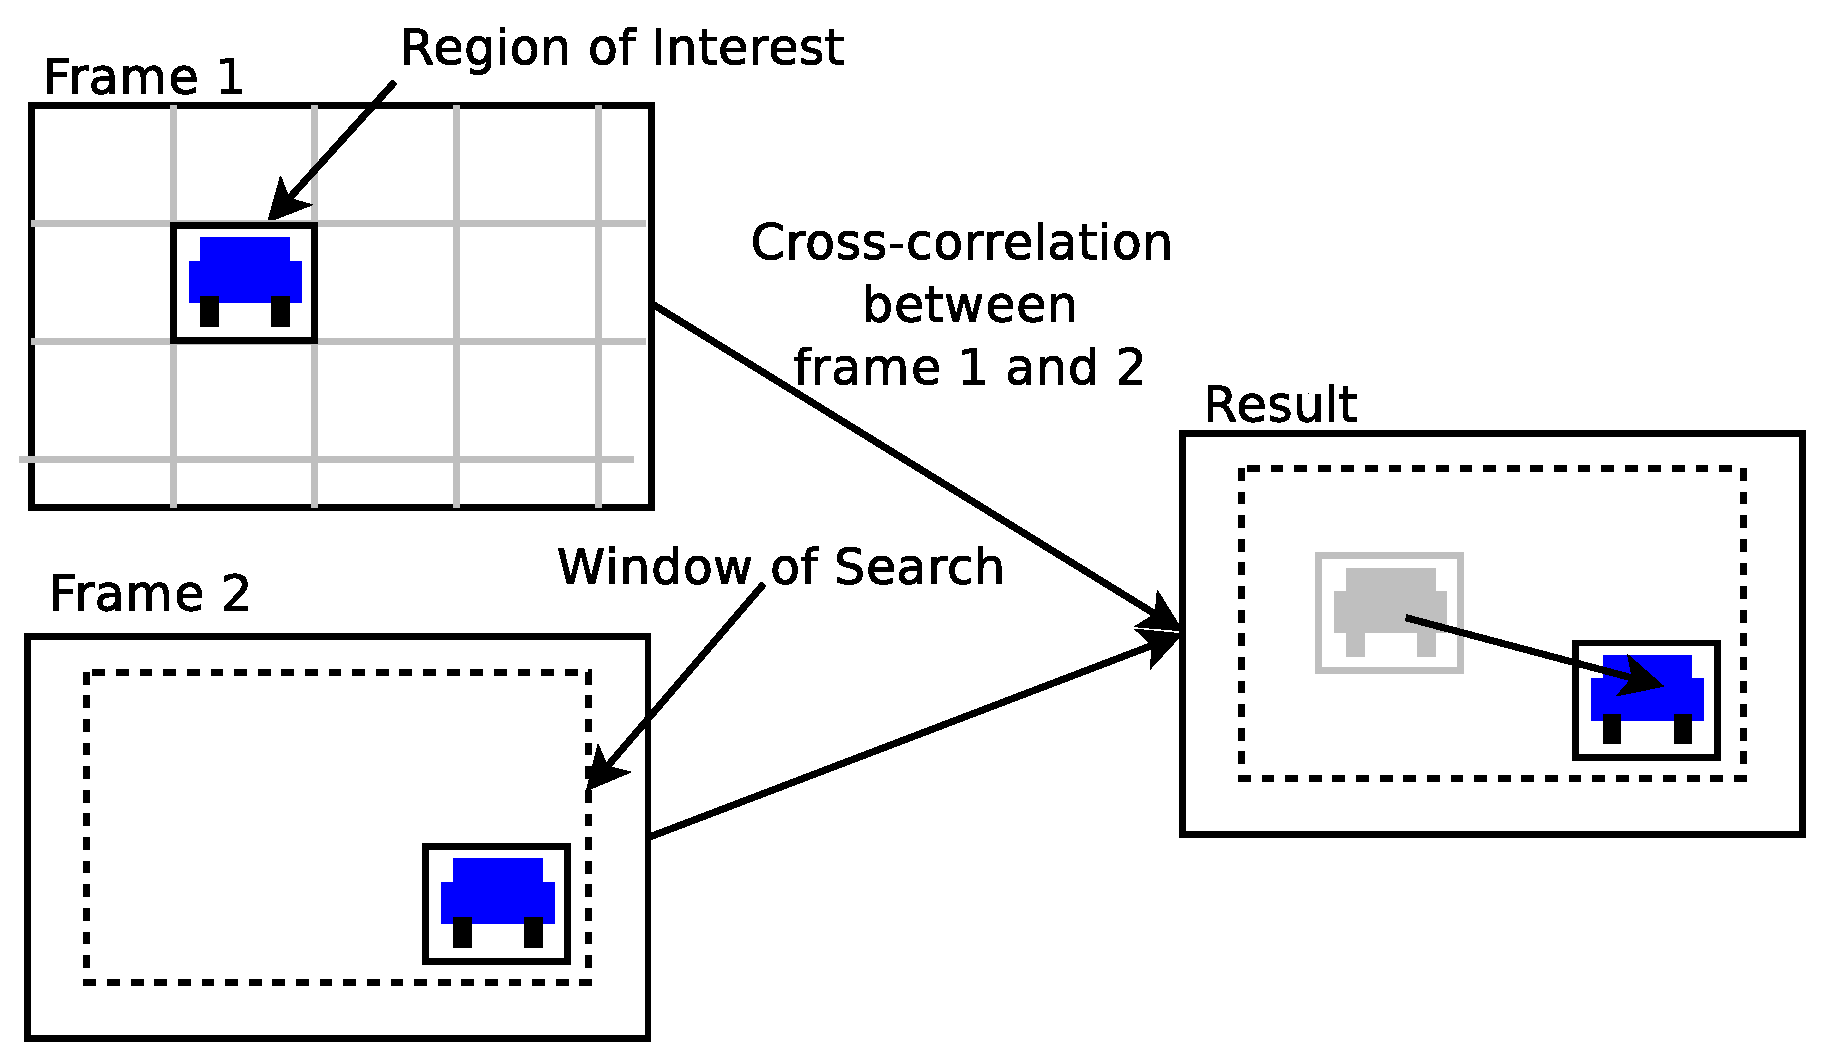
\includegraphics[width=\columnwidth]{images/explanationPIV.eps}
\caption{The PIV operation comparing two frames}
\label{fig:twoframes}
\end{figure}

The Fig. \ref{fig:twoframes} illustrates how $PIV$ works and demonstrates the relation between Region of Interest ($ROI$) and 
Window of Search ($WOS$). where $WOS$ is a region where the target will be searched and consequently $WOS$ must involve ROI. 
$WOS$ doesn't fill necessary whole image. If $WOS$ is large, we have an augment of computing but 
if $WOS$ is too small, target in high velocity has more chances to be lost. In our application, 
we determine $WOS$ from $1.5$ of $ROI$. For example, if ROI is $200\times300$ so we have WOS of $300\times450$. 
This consideration can be tuned by tests, by example considering environments with objects
of low velocity (permitted velocity in cities and roads).

\begin{figure}[H]
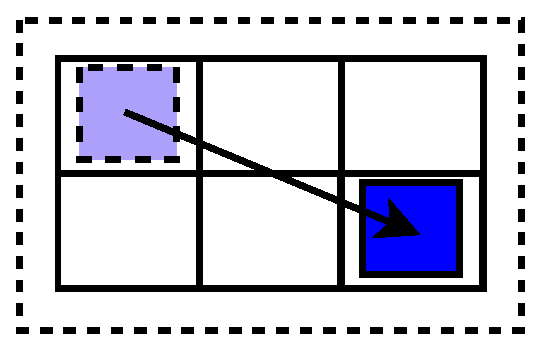
\includegraphics[width=\columnwidth]{images/WOSdivided.eps}
\caption{The $ROI$ is searched in the $ROI$ on windows of same dimensions. }
\label{fig:WOSdivided}
\end{figure}

$ROI$ is one of most important part of $PIV$, because it contains target. An Analysis Region ($AR$)
of same dimension of $ROI$ is displaced
along of whole $WOS$ in frame $2$, like showed in Fig. \ref{fig:WOSdivided}. Comparisons are done among regions between frames and are 
assigned values. 
When process finishes, the more height value refers the new place of $ROI$. It means that target displaced of a point in 
frame $1$ to another in frame $2$.

\end{comment}

%%%%%%%%%%%%%%%%%%%%%%%%%%%%%%%%%%%%%%%%%%%%%portugues%%%%%%%%%%%%%%%%%%%%%%%%%%%%%%%%%%%%%%%%%%%%%%%%%%%%%%%%%%%%%

\subsection{PARTICLE IMAGE VELOCIMETRY - PIV}

O $PIV$ é uma técnica que determina um campo de velocidade de objetos dentro de um fluxo de imagem \cite{Bastiaans}.
O resultado do $PIV$ é dado por um campo de vetor que representa a direção, sentido e intensidade de velocidade de cada 
partícula. Além disso, pode ser usado para acompanhar objetos dentro de um fluxo de imagens.

O $PIV$ divide a imagem em diferentes possíveis regiões onde o objeto pode ser encontrado. A região que contém o objeto de 
interesse é correlacionada com a próxima imagem. Após ser encontrado sua correspondente, um vetor é traçado do ponto inicial
até a região encontrada. Assim, evidencia-se um deslocamento entre uma imagem e outra, aplicando a derivada 
obtém-se a estimativa da velocidade relativa.

\begin{figure}[H]
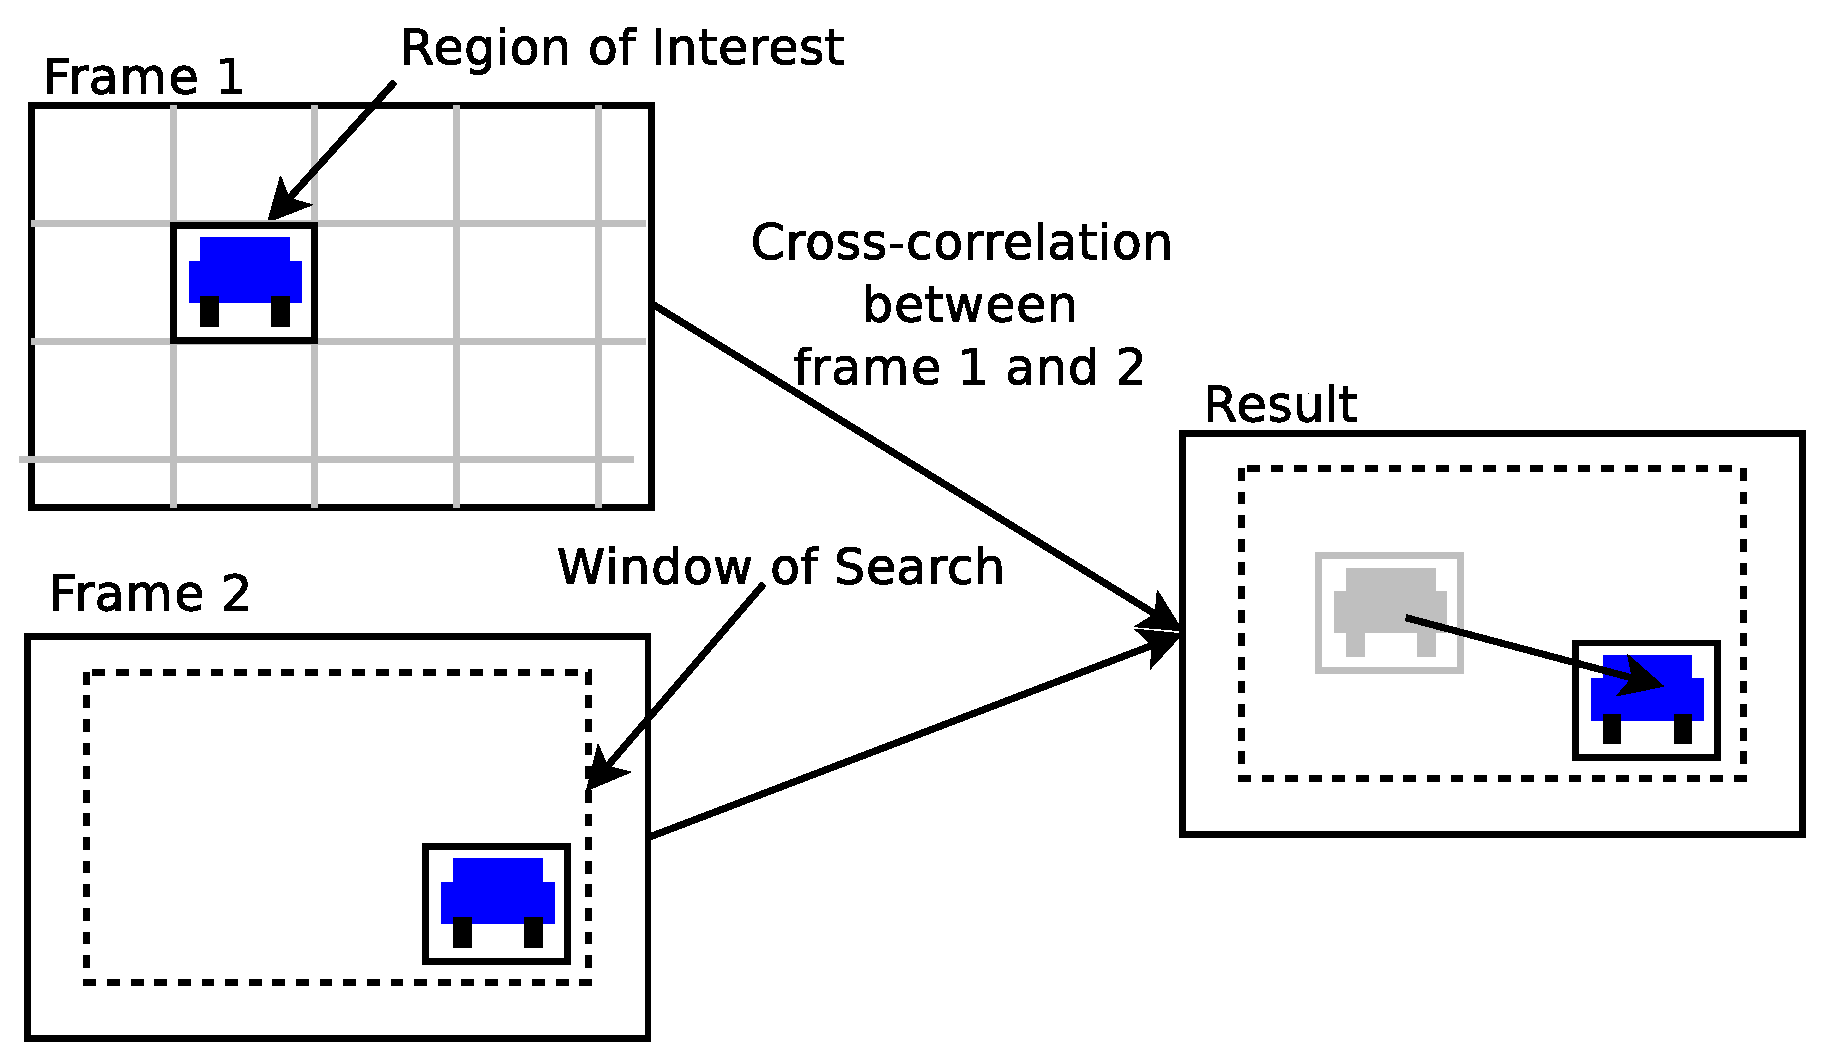
\includegraphics[width=\columnwidth]{images/explanationPIV.eps}
\caption{Funcionamento do $PIV$, comparando duas imagens.}
\label{fig:twoframes}
\end{figure}

A figura \ref{fig:twoframes} ilustra como $PIV$ funciona, demonstrando a relação entre a região de interesse ($ROI$) e 
a janela de busca ($WOS$). $WOS$ é a região onde o objeto pode ser encontrado sendo proporcional ao tamanho do $ROI$.
O $WOS$ é definido $1.5$ o tamanho do $ROI$. Por exemplo, se o $ROI$ tem dimensão $200\times300$, então o $WOS$ terá $300\times450$.
Essa consideração foi tomada a partir dos testes feitos e levando em conta os limites de velocidades permitidos em 
cidades e rodovias.


\begin{figure}[H]
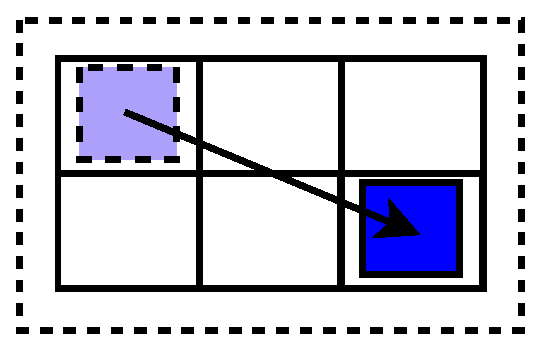
\includegraphics[width=\columnwidth]{images/WOSdivided.eps}
\caption{O $WOS$ é o espaço pelo qual o $ROI$ será procurado.}
\label{fig:WOSdivided}
\end{figure}

$ROI$ é uma das partes mais importantes do $PIV$, pois ele contém o objeto de interesse. Uma região de análise
($AR$) da mesma dimensão do $ROI$ é percorrida pelo $WOS$ na imagem 2, como mostrado na figura \ref{fig:WOSdivided}.
As comparações são feitas entre as regiões de ambas imagens e calculado um valor para essa comparação, quando o processo termina o valor
maior da correlação é a nova posição do objeto. Deste modo, traça-se um vetor do ponto inicial ($ROI$ na imagem 1) até o ponto final
($ROI$ na imagem 2).



\section{DESCRIÇÃO DO SISTEMA}
%The purpose of this algorithm is to make a (3D) tracking system, producing position informations 
about the followed target.
These informations will be relevant to define parameters 
as: the relative velocity, the factor of approaching and of departure.

The proposed algorithm is shown in the Fig. \ref{fig:system};
this begin with a key frame image where a initial Region Of Interest ($ROI$) is determined; 
the system then receive a stream of image frames and the tracking system 
enters in looping to follow the target in the next frames.
In this case, to difference of $PIV$, the compared images are 
the current image in the image stream and the current $ROI$.

\begin{figure}[bhp]
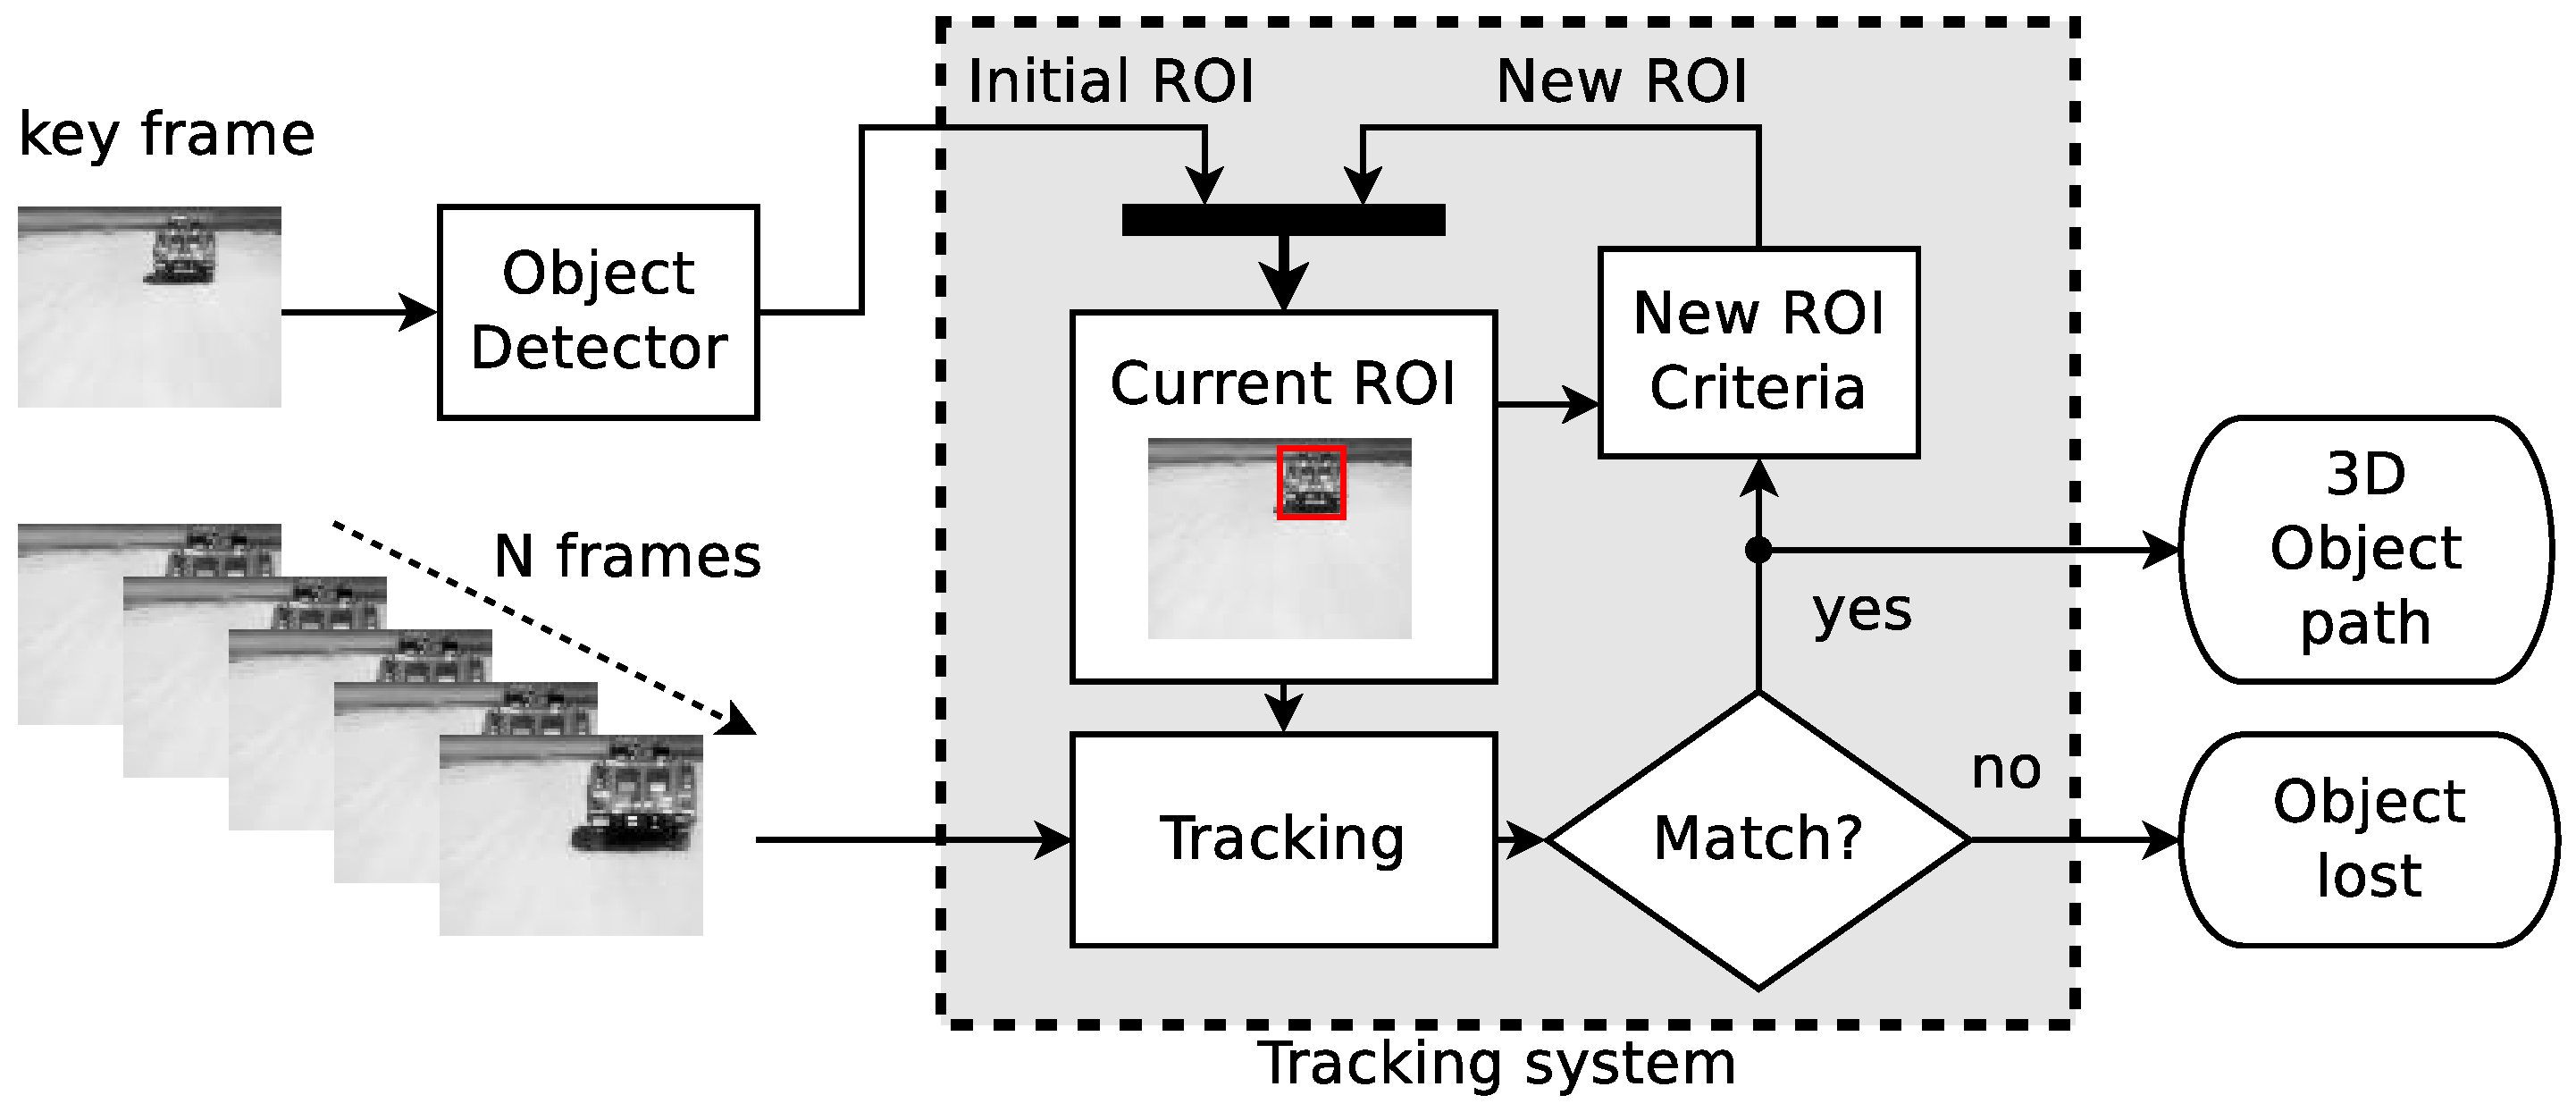
\includegraphics[width=\columnwidth]{images/figure1-diagram1.eps}
\caption{With the current $ROI$ selected, a highest value of $PCC$, between the $ROI$ 
and the Window Of Search ($WOS$) of current frame, identifies the target; 
the result of search is a displacement vector
between the first and last position of object. 
After, this processing is made again to the next frames.}
\label{fig:system}
\end{figure}

In a 2 dimensional analysis, the tracked objects given us information about your horizontal 
and vertical position, and your relative perpendicular velocity respect to the observer.
When the target is analyzed in 3 dimensions, 
the initial $ROI$ has the position $(x=x_0,y=x_0,d=d_0=1)$;
where, $x_0$ and $y_0$ represent a position (horizontal and vertical) in the analyzed image,
and $d_0=1$ represents the initial depth position of object in the $ROI$ (normalized by definition to $1.0$).
Thus, all the results of depth will be relatives to this value, 
In this sense only can be calculated, relative values of
velocity and the factor of approaching or departure. 

%Diagrama1
 %A gente vai explicar o algoritmo como uma caixa fechada , que coisa entra e que coisa sai
 %e os parametros a sintonizar.
 % como usar ele quando implementado, como se fosse uma caixa preta.
 %%FAZER

\section{DESCRIÇÃO DO ALGORITMO}
 
%DiagramaX
%\subsection{ERROR REDUCTION}

In this section, we discuss about the error in analysis of the images. In this sense,
we can see that, the targets have different forms; however, 
a $ROI$ ever will have a rectangular form, so that certain areas will be more important of identify inside of $ROI$.
In Fig. \ref{fig:erroridentified}, there are some areas close of edges that target not occupies; they are
considered like error areas.

\begin{figure}[H]
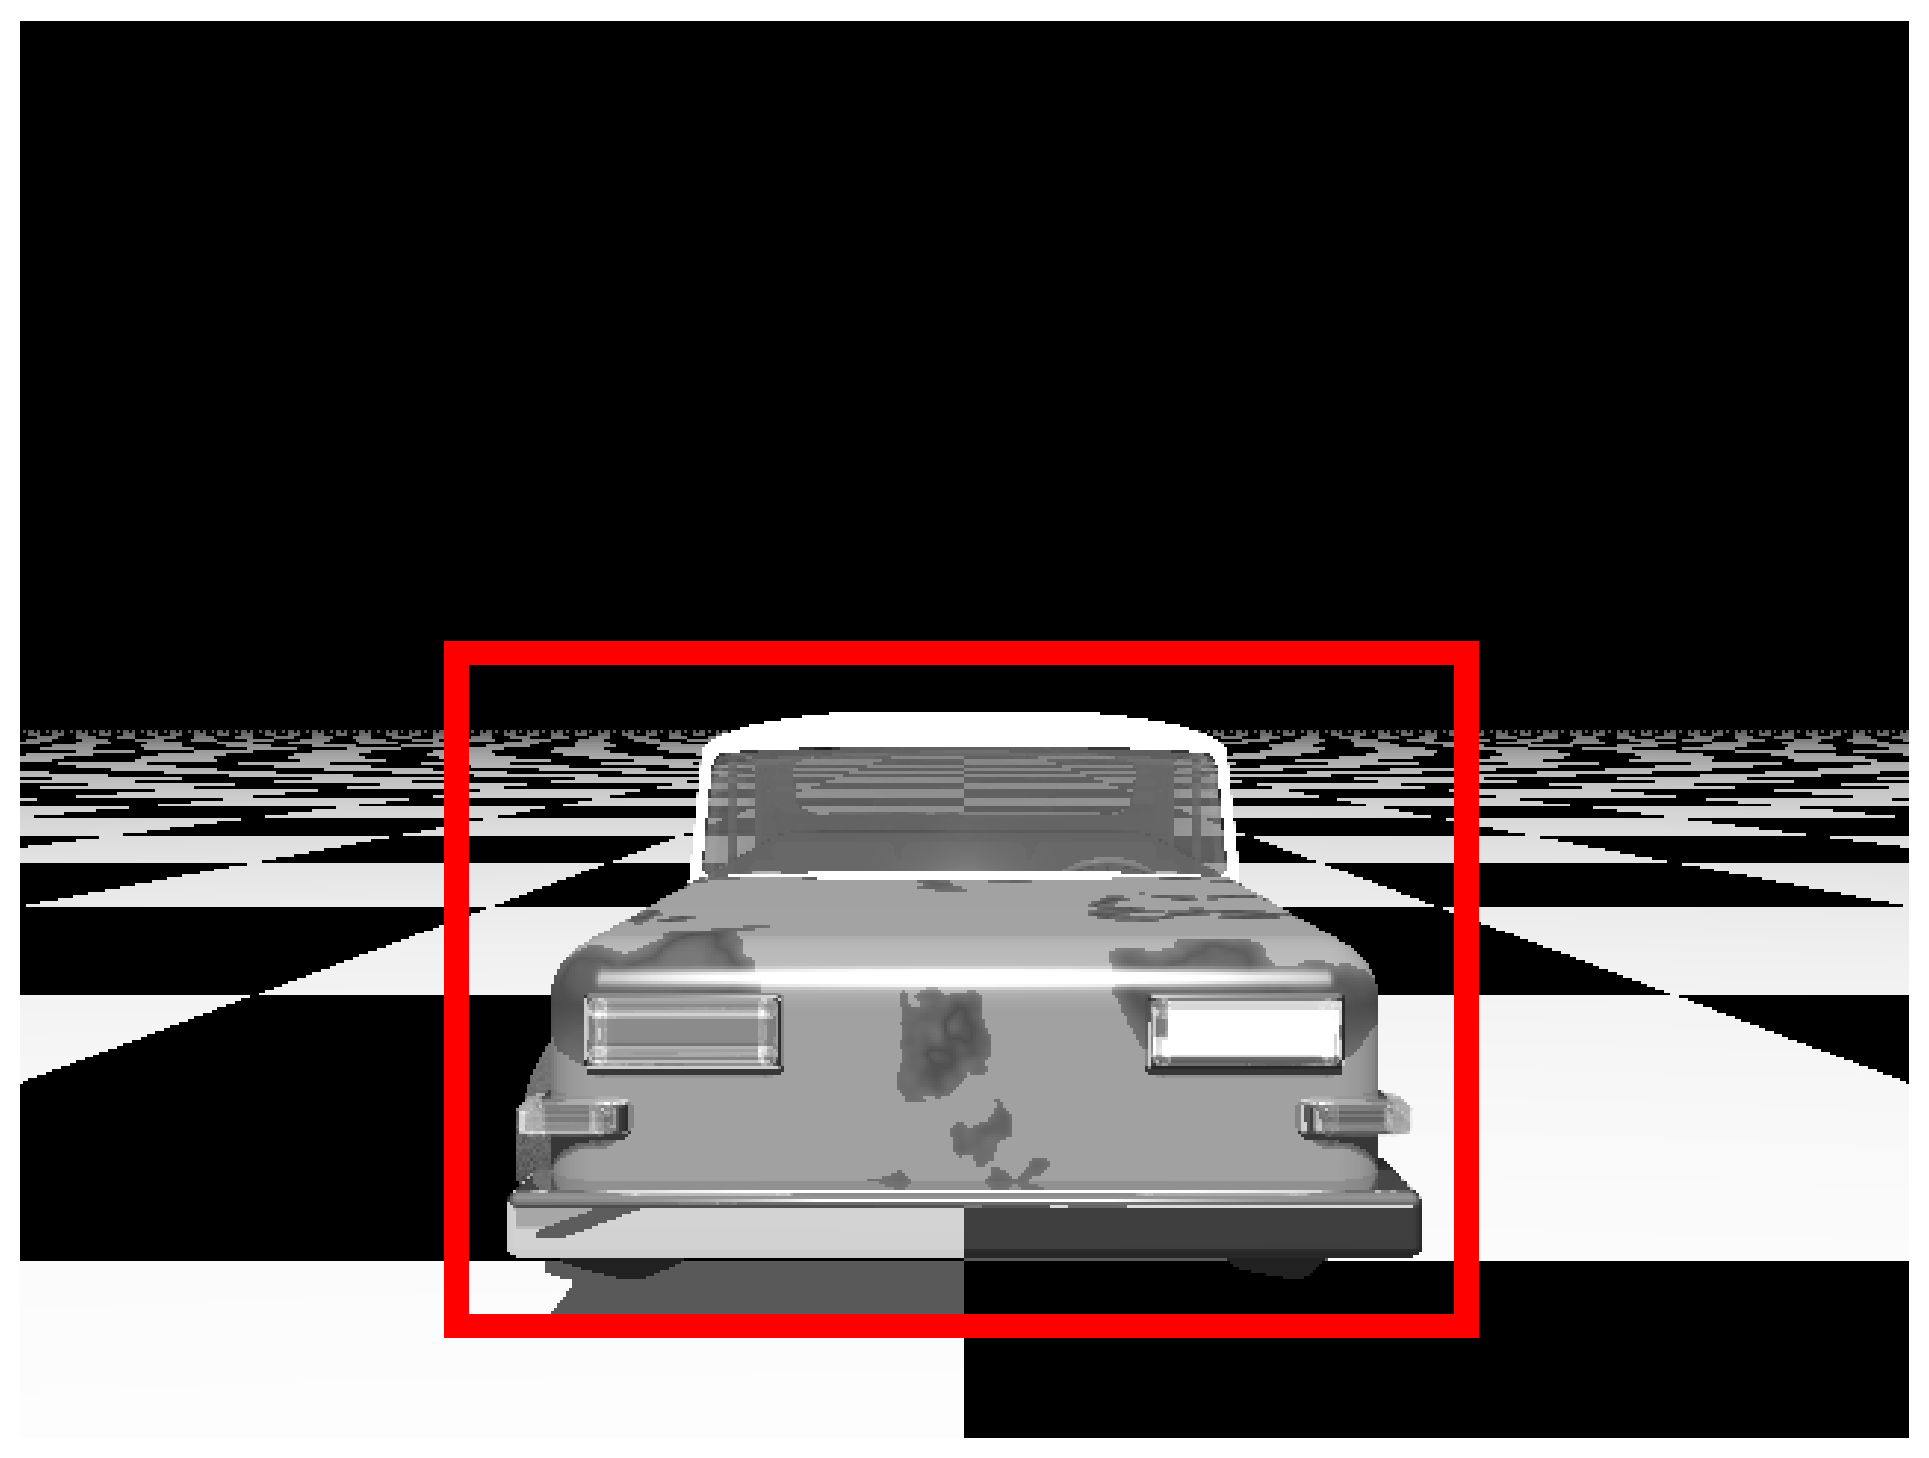
\includegraphics[width=\columnwidth]{images/imageError.eps}
\caption{Illustration of $ROI$ with error areas close of edge.}
\label{fig:erroridentified}
\end{figure}

Whereas, two matrix with the same dimensions can be compared using $PCC$; 
this method of comparison doesn't generate data over equals frames.
On the other hand, if the frames have a proportional change in the relation its values. 
Thus, a high percentage of error area when compared with the target area 
may decrease the correlation level between frames and target is considered out of scene. 
We decide solve this problem using a weighting matrix mask over the analyzed regions, 
before the calculus of $PCC$. This can be seen in the Fig. \ref{fig:errorpondered}.
\begin{figure}[H]
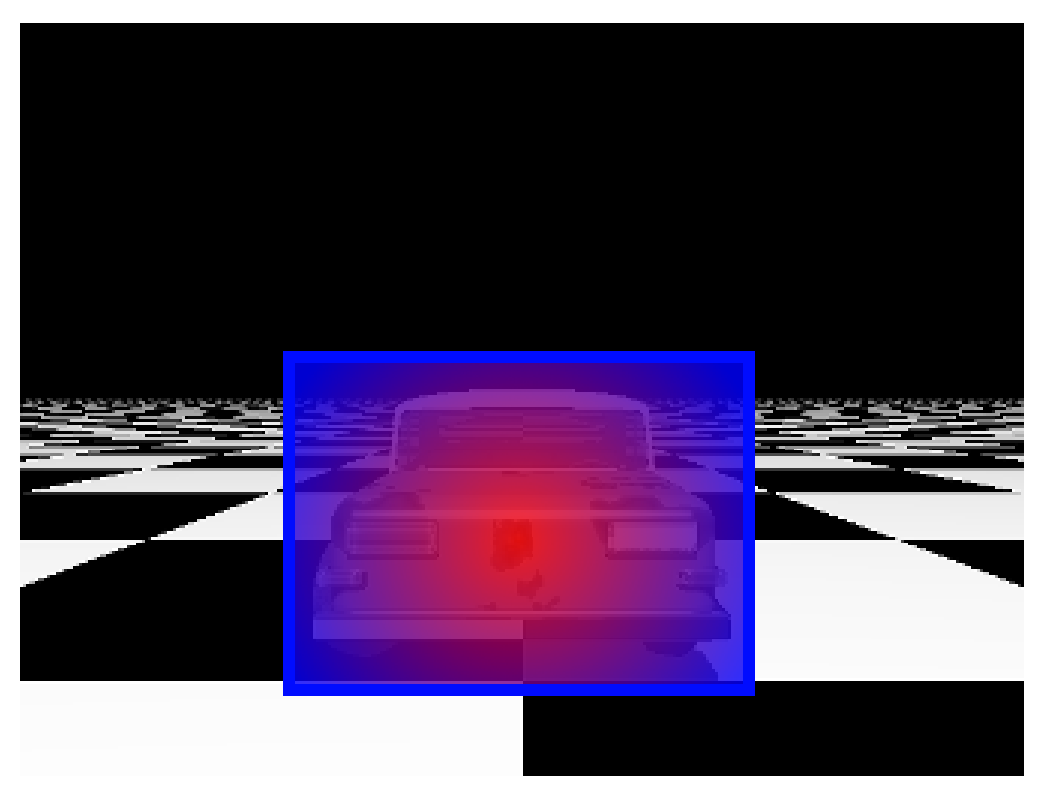
\includegraphics[width=\columnwidth]{images/imageErrorcontroled.eps}
\caption{Illustration of points of most importance (red) and points less importance (blue) in correlation.}
\label{fig:errorpondered}
\end{figure}
Where, points close of edge (in blue color) have less importance, 
points close of center of image (in red color), probably are on the target, and consequently
these points will have more importance. 

Thus, the $Q(x,y)$ value showed in the Eq. (\ref{eq:Q}), 
\begin{equation}\label{eq:Q}
 Q(x,y) = \sqrt{e^{ -\frac{|x-\mu_X|^3}{\sigma_X^3}-\frac{|y-\mu_Y|^3}{\sigma_Y^3}  }},
\end{equation}
represents a value, in the line $x$ and column $y$, on the weighting matrix mask $Q$,
where $\mu_X=H/2$, $\mu_Y=W/2$, $\sigma_X=H/3$ and $\sigma_Y=W/3$; being $H$ and $W$
the height and the width, respectively, in the analysis region.

Finally, similarly to seen in the Eq. (\ref{eq:PCC}), we multiply the matrix $Q$, 
element by element, over the analysis regions
$A$ and $B$ to calculate the $r_P$ weighted correlation coefficient, 
\begin{equation}\label{eq:rw}
 r_Q = PCC(Q~A, Q~B).
\end{equation}


 %%FAZER
\begin{comment}

\subsection{MULTI-SCALE MATCH CRITERION}
In the presented algorithm, the match criterion to track the target is based on the $PIV$ technique. 
Region of Interesting ($ROI$) and Window Of Search ($WOS$) are defined. A target (object) is identified 
from the highest value of correlation ($CCP$) between selected $ROI$ and an analysis region in the $WOS$,
which determines an object's location.

Fig. \ref{fig:multires}(a) shows an application in two dimensions, where
the regions are compared with a ROI using the same scale.

The Fig. \ref{fig:multires}(b) reveals how the dimension of depth was included and
the search is made in different scales (layers). Similarly to the two dimension case, 
in three dimensions the target is also found through the highest $CCP$, but the object found may be 
bigger or smaller than the last target found.

\begin{figure}[H]
\centering
  \subfloat[]{\label{subfig:(a)} 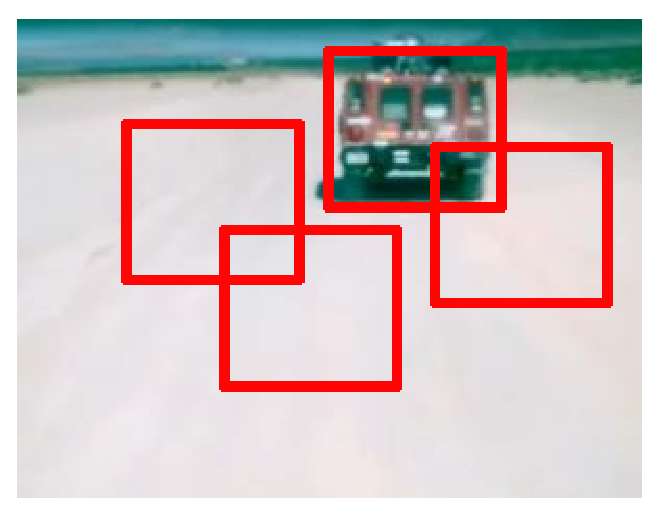
\includegraphics[width=.5\columnwidth]{images/figure2a.eps}}
  \subfloat[]{\label{subfig:(b)} 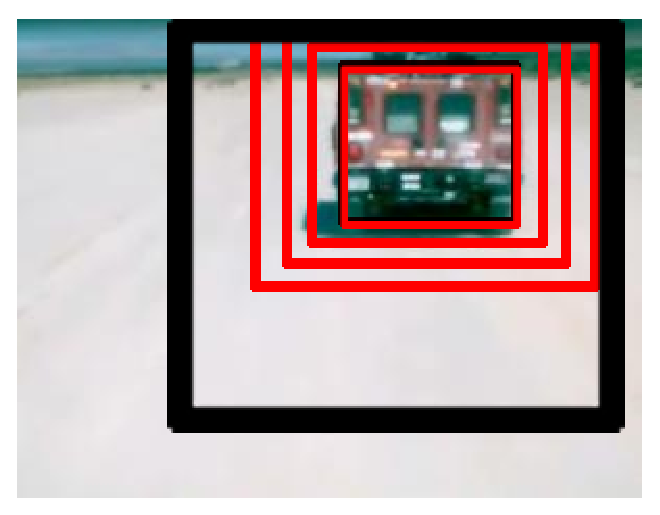
\includegraphics[width=.5\columnwidth]{images/figure2b.eps}}
  \caption{The red boxes show the analyzed regions and the black boxes represent the $WOS$. 
  (a) The regions are compared with a $ROI$ using the same scale. 
  (b) The regions are compared with a $ROI$ using different scales.}
  \label{fig:multires}
\end{figure}

The Algorithm \ref{alg:multires} describes the method explicated in the 
Fig. \ref{fig:multires}(b), It is represented by the function 
$multiscale\_match\_criterion()$ and It is used in the Algorithm \ref{alg:system}.

\begin{algorithm}
 \KwData{A $ROI$, your position $P_0$ and an image frame $I_i$. }
 \KwResult{The best matched analysis region, $AR$, your position 
 $P_{max}$ and the correlation value,$r_{max}$, with the $ROI$. }
 ~\\
 $W$: Width of $ROI$\;
 $H$: Height of $ROI$\;
 $L$: Search arm in pixels (defined by the user)\;
 $\alpha \leftarrow 0.8$\;
 $r_{max} \leftarrow -1.0$\;
 ~\\
    \While{$0.8 \leq \alpha \leq 1.4 $}{
      
      $A \leftarrow get\_corr\_matrix(ROI,P_0,\alpha,L,I_i)$\;

      $p_i$: position $(x_i,y_i)$ of maximum value in $A$\;

      $r \leftarrow A(p_i)$\;

      \If{$r > r_{max}$}{
	$r_{max} \leftarrow r$\;
	$P_{max} \leftarrow P_0 +p_i-(L,L)$\;
	$\alpha_{max} \leftarrow \alpha$\;
      }
      ~\\
      $\alpha \leftarrow \alpha +0.05$\;
    }
    
$AR$: Region in $I_i$, at point $P_{max}$, with size $\alpha W$ by $\alpha H$\;      
\Return $\{AR,P_{max},r_{max}\}$\;
~\\
\caption{$multiscale\_match\_criterion(ROI,P_0,I_i)$ function.}
\label{alg:multires}
\end{algorithm}

We can see that the Algorithm \ref{alg:multires} uses internally
the function $get\_corr\_matrix()$, this function returns a matrix 
with the correlation values of $ROI$ with the analyses of regions
inside the $WOS$ around the central point $P_0$. 
All the procedure of this function can be seen detailed in the Algorithm \ref{alg:multires2}.

\begin{algorithm}
 \KwData{A $ROI$, your position $P_0$, a departure factor $\alpha$, the search arm 
 $L$ and an image frame $I_i$. }
 \KwResult{The correlation matrix $A$, compound around the point $P_0$ of $I_i$. }
 ~\\
 $W$: Width of $ROI$\;
 $H$: Height of $ROI$\;
 $lin_0$: The first term of $P_0$\;
 $col_0$: The second term of $P_0$\;
 $A$: Creates a square matrix of $2L+1$ pixels by side and fill it with zeros\;

 ~\\
    \For{$-L \leq lin \leq L$}{
    \For{$-L \leq col \leq L$}{
      $AR$: Region in $I_i$, at point $(lin_0+lin,col_0+col)$, with size $\alpha W$ by $\alpha H$\;
      $AR \leftarrow $ rescale $AR$ to $ROI$ size\;
      
      $Q$ is filled according the Eq. (\ref{eq:Q})\;
      $A(L+lin,L+col) \leftarrow CCP(Q\times ROI,Q\times AR)$\;

    }
    }
    
\Return $A$\;
~\\
\caption{$get\_corr\_matrix(ROI,P_0,\alpha,L,I_i)$ function.}
\label{alg:multires2}
\end{algorithm}


%onde estava, onde esta agora
%que tamanho tinha que tamanho tem.

\end{comment}

%%%%%%%%%%%%%%%%%%%%%%%%%%%%%%%%%%%%%%%%%%%%%%%%%portugues%%%%%%%%%%%%%%%%%%%%%%%%%%%%%%%%%%%%%%%%%%%%%%%%%%

\subsection{Critério de busca em camadas}

O critério de busca do objeto de interesse está baseada na técnica $PIV$; 
consequentemente, é necessário definir alguns parâmetros para executar  
este algoritmo. Assim nos temos, a região de interesse ou $ROI$ 
 que é a região ou porção da imagem que contém
o objeto de interesse, também precisamos uma janela de busca ou $WOS$
que é a região onde serão analisadas regiões para identificar a $ROI$. 
Na técnica $PIV$ tradicional, quando é analisada uma imagen, 
a posição da $ROI$ na imagem é obtida a partir 
da posição da região analisada na imagem com o valor de $CCP$ mais próximo de $1.0$,
quando comparado com a $ROI$. 
Essa análise consiste na divisão da $WOS$ em regiões de analises que sejam do tamanho da $ROI$, pois o $CCP$
compara imagens do mesmo tamanho.

A Figura \ref{fig:multires}(a) mostra a aplicação da técnica $PIV$ 
para duas dimensões (tradicional), onde as regiões de analises na $WOS$
são comparadas com a $ROI$. 
A Figura \ref{fig:multires}(b) representa uma aplicação em 3 dimensões da técnica $PIV$. 
Neste ponto, inclui-se camadas, estas consistem na diminuição e aumento da regiões de analises os quais 
contemplam casos de afastamento e aproximação do objeto, respectivamente.

\begin{figure}[H]
\centering
  \subfloat[]{\label{subfig:(a)} 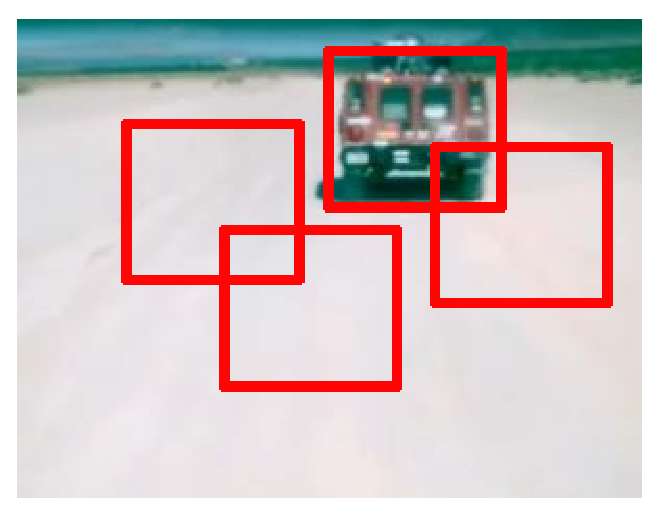
\includegraphics[width=.5\columnwidth]{images/figure2a.eps}}
  \subfloat[]{\label{subfig:(b)} 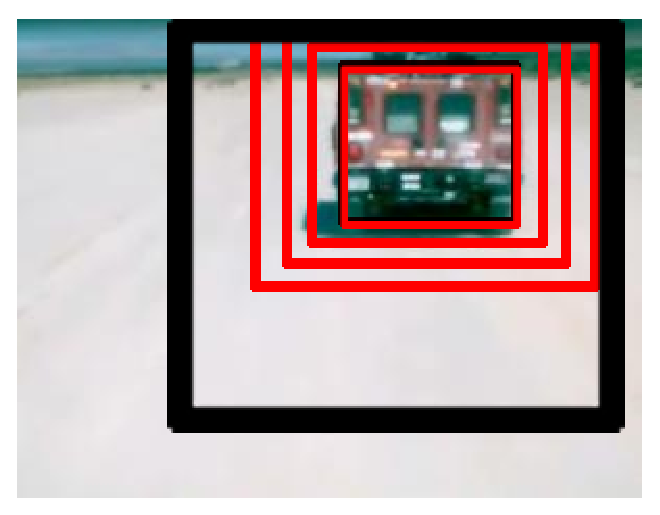
\includegraphics[width=.5\columnwidth]{images/figure2b.eps}}
  \caption{Os retângulos vermelhos mostram as regiões analisadas e o retângulo preto representa o $WOS$. 
  (a) As regiões de analises do $WOS$ são comparadas com o $ROI$ em uma única camada. 
  (b) As regiões de analises do $WOS$ sendo comparadas com $ROI$ de diferentes escalas é dizer múltiplas camadas.}
  \label{fig:multires}
\end{figure}

O algoritmo \ref{alg:multires} descreve o método usado na Figura \ref{fig:multires}(b), o qual
está representado pela função $multiscale\_match\_criterion()$ no algoritmo \ref{alg:system}.
\begin{algorithm}
 \KwData{ $ROI$, posição $P_{i-1}$ do objeto de interesse na imagem $I_{i-1}$ e a imagem $I_i$. }
 \KwResult{A região $AR$ com a mais alta correlação, a posição 
 $P_{max}$ e o valor $r_{max}$ da correlação com a $ROI$. }
 ~\\
 $W$: Width of $ROI$\;
 $H$: Height of $ROI$\;
 $L$: Search arm in pixels (defined by the user)\;
 $\alpha \leftarrow 0.8$\;
 $r_{max} \leftarrow -1.0$\;
 ~\\
    \While{$0.8 \leq \alpha \leq 1.4 $}{
      
      $A \leftarrow get\_corr\_matrix(ROI,P_{i-1},\alpha,L,I_i)$\;

      $p_i$: position $(x_i,y_i)$ of maximum value in $A$\;

      $r \leftarrow A(p_i)$\;

      \If{$r > r_{max}$}{
	$r_{max} \leftarrow r$\;
	$P_{max} \leftarrow P_{ROI} +p_i-(L,L)$\;
	$\alpha_{max} \leftarrow \alpha$\;
      }
      ~\\
      $\alpha \leftarrow \alpha +0.05$\;
    }
    
$AR$: Region in $I_i$, at point $P_{max}$, with size $\alpha_{max} W$ by $\alpha_{max} H$\;      
\Return $\{AR,P_{max},r_{max}\}$\;
~\\
\caption{$multiscale\_match\_criterion(ROI,P_{i-1},I_i)$ function.}
\label{alg:multires}
\end{algorithm}
O algoritmo \ref{alg:multires} usa internamente a função $get\_corr\_matrix()$,
esta função tem como saída uma matriz com os valores da correlação da $ROI$ e as regiões de analises na $WOS$
em torno ao ponto $P_{i-1}$. Todos os processos da função $get\_corr\_matrix()$ são detalhados no algoritmo
\ref{alg:multires2},
\begin{algorithm}
 \KwData{$ROI$, posição $P_{i-1}$ sendo este o centro da $WOS$, 
 fator de aproximação $\alpha$ relativa à distancia $d_{ROI}$, braço de busca 
 $L$ e a imagem $I_i$. }
 \KwResult{A matriz de correlação $A$, da regiões ao redor do ponto $P_{i-1}$ da imagem $I_i$. }
 ~\\
 $W$: Width of $ROI$\;
 $H$: Height of $ROI$\;
 $lin_c$: The first term of $P_{i-1}$\;
 $col_c$: The second term of $P_{i-1}$\;
 $A$: Creates a square matrix of $2L+1$ pixels by side and fill it with zeros\;

 ~\\
    \For{$-L \leq lin \leq L$}{
    \For{$-L \leq col \leq L$}{
      $AR$: Region in $I_i$, at point $(lin_c+lin,col_c+col)$, with size $\alpha W$ by $\alpha H$\;
      $AR \leftarrow $ rescale $AR$ to $ROI$ size\;
      
      $Q$ is filled according the Eq. (\ref{eq:Q})\;
      $A(L+lin,L+col) \leftarrow CCP(Q\times ROI,Q\times AR)$\;

    }
    }
    
\Return $A$\;
~\\
\caption{$get\_corr\_matrix(ROI,P_{i-1},\alpha,L,I_i)$ function.}
\label{alg:multires2}
\end{algorithm}

\begin{comment}
\subsubsection{MULTI-SCALE 3D INTERPRETATION}
To understand this technique we need to analyse the same target in 
two different positions, as in Fig. \ref{fig:multiscale3d}.

\begin{figure}[H]
\centering
  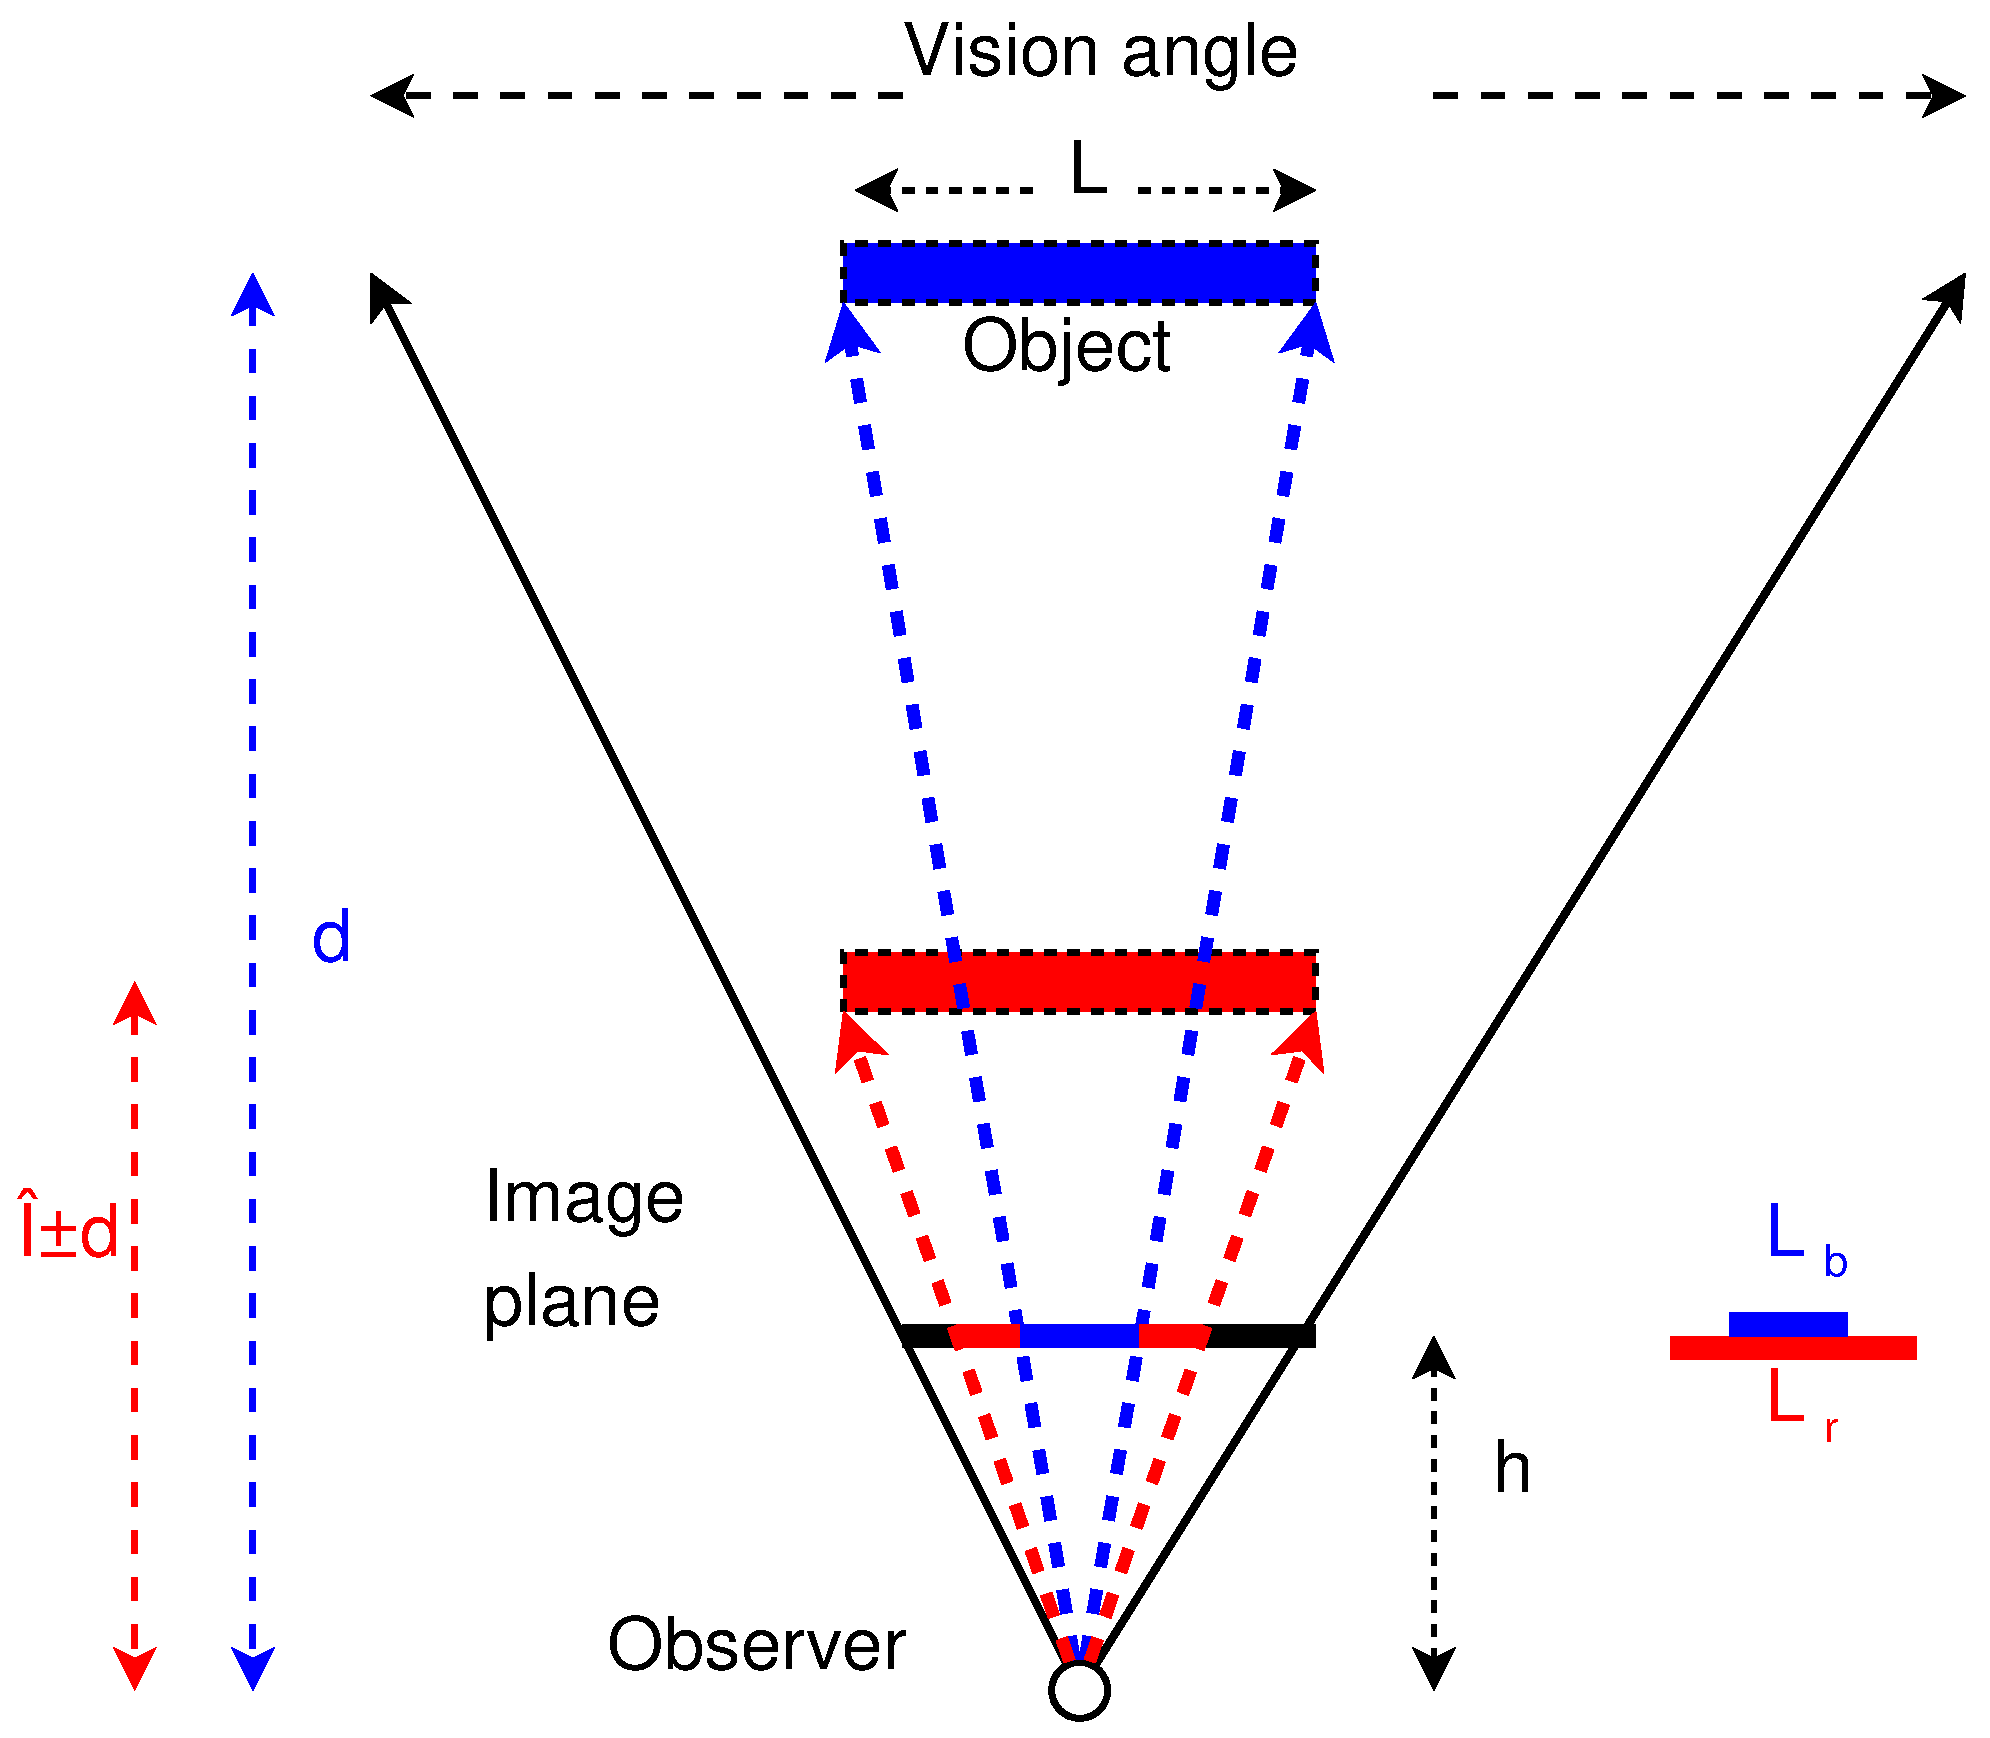
\includegraphics[width=.7\columnwidth]{images/Diagrama3.eps}
  \caption{The multi-scale tracking.}
  \label{fig:multiscale3d}
\end{figure}

Fig.\ref{fig:multiscale3d} shows the same target at two different distances $d$ and $\alpha d$, respectively, in blue and red.
The image plane is located at a distance $h$ of the observer.
The projections of objects, in blue and red, are labelled in the image as
$L_b$ and $L_r$, respectively. Making a simple inspection in the
formed triangles, we can see that $\frac{h}{d}=\frac{L_b}{L}$ and 
$\frac{h}{\alpha d}=\frac{L_r}{L}$, then $L_b/\alpha= L_r$. 
From the point of view of the observer, this implies that when a target 
was located at a distance $d$ at a time $t_0$,  and is moved to a distance $\alpha d$ at a time $t_1$, 
the width of the target in the image plane is altered by a factor of 1/$\alpha$, 
and consequently its area is altered by a factor of 1/$\alpha^2$.

The search criterion of objects uses different discrete values of $\alpha$, so that 
the algorithm tracks nearest objects with $\alpha<1$ and farthest objects  with $\alpha>1$.

%usa Multi-resolution match criteria e explica isso dos tamanhos

\subsubsection{DEPARTURE FACTOR - RELATIVE VELOCITY}
The departure factor is a dimensionless number related to the rate of approach 
or departure of a target to the observer. The factor
is determined in Eq. (\ref{eq:relarea}),

\begin{equation}\label{eq:relarea}
f_a \equiv \alpha^2 \equiv \frac{Area_r}{Area_f} 
\end{equation}

where $f_a$ and $\alpha$ are defined as factor area and departure factor, 
respectively; $Area_r$ is the ROI area and $Area_f$ 
is the analyzed region in the current image frame.

Thus, knowing $\alpha$, if we consider that the target in the $ROI$ was to a distance $d_0$,
then the target in the analysis region will be to a distance of $\alpha d_0$ (or $\sqrt{f_a} d_0$).
So that, each $i-th$ frame will have its own $\alpha_i$ value; where, $d_i=\alpha_i d_0$.

The departure factor, $\alpha_i$, has two interpretations: if the rate of departure increases quickly, 
this  means that the target is departing. If the factor decreases, the 
target is approaching.

The relative velocity is using a simple equation of kinematic in physics:
\begin{equation}
 v_i = \frac{\Delta s}{\Delta t}= \frac{s_i-s_{i-1}}{\Delta t}.
\end{equation}

where the vector $v_i$ represents the relative velocity in the i-th image frame, 
$s_i=(x_i,y_i,d_i)$ is the position of match in the i-th image frame
and $\Delta t$ is the sampling time between image frames.
Additionally, we call velocity of departure factor, $v^d_i$, 
the scalar number which represents the depth component
of the vector $v_i$.

The calculated  $v^d_i$ value is relative, for the simple reason that the distance (depth) between the 
camera (observer) and the target in the instance i-th will be referenced to $d_0$, 
given that the distance of the initial $ROI$ is established by definition to 1.
Finally, in all cases, the position $s_i$ is relative to the observer (a moving reference system).

\end{comment}

%%%%%%%%%%%%%%%%%%%%%%%%%%%%%%%portugues%%%%%%%%%%%%%%%%%%%%%%%%%%%%%%%%%%%%%%%%%%%%%%%


\subsubsection{Interpretação da busca em camadas- 3D}

Para compreender essa técnia é necessário analisar o objeto 
em diferentes posições, como mostrado na Fig. \ref{fig:multiscale3d}.

\begin{figure}[H]
\centering
  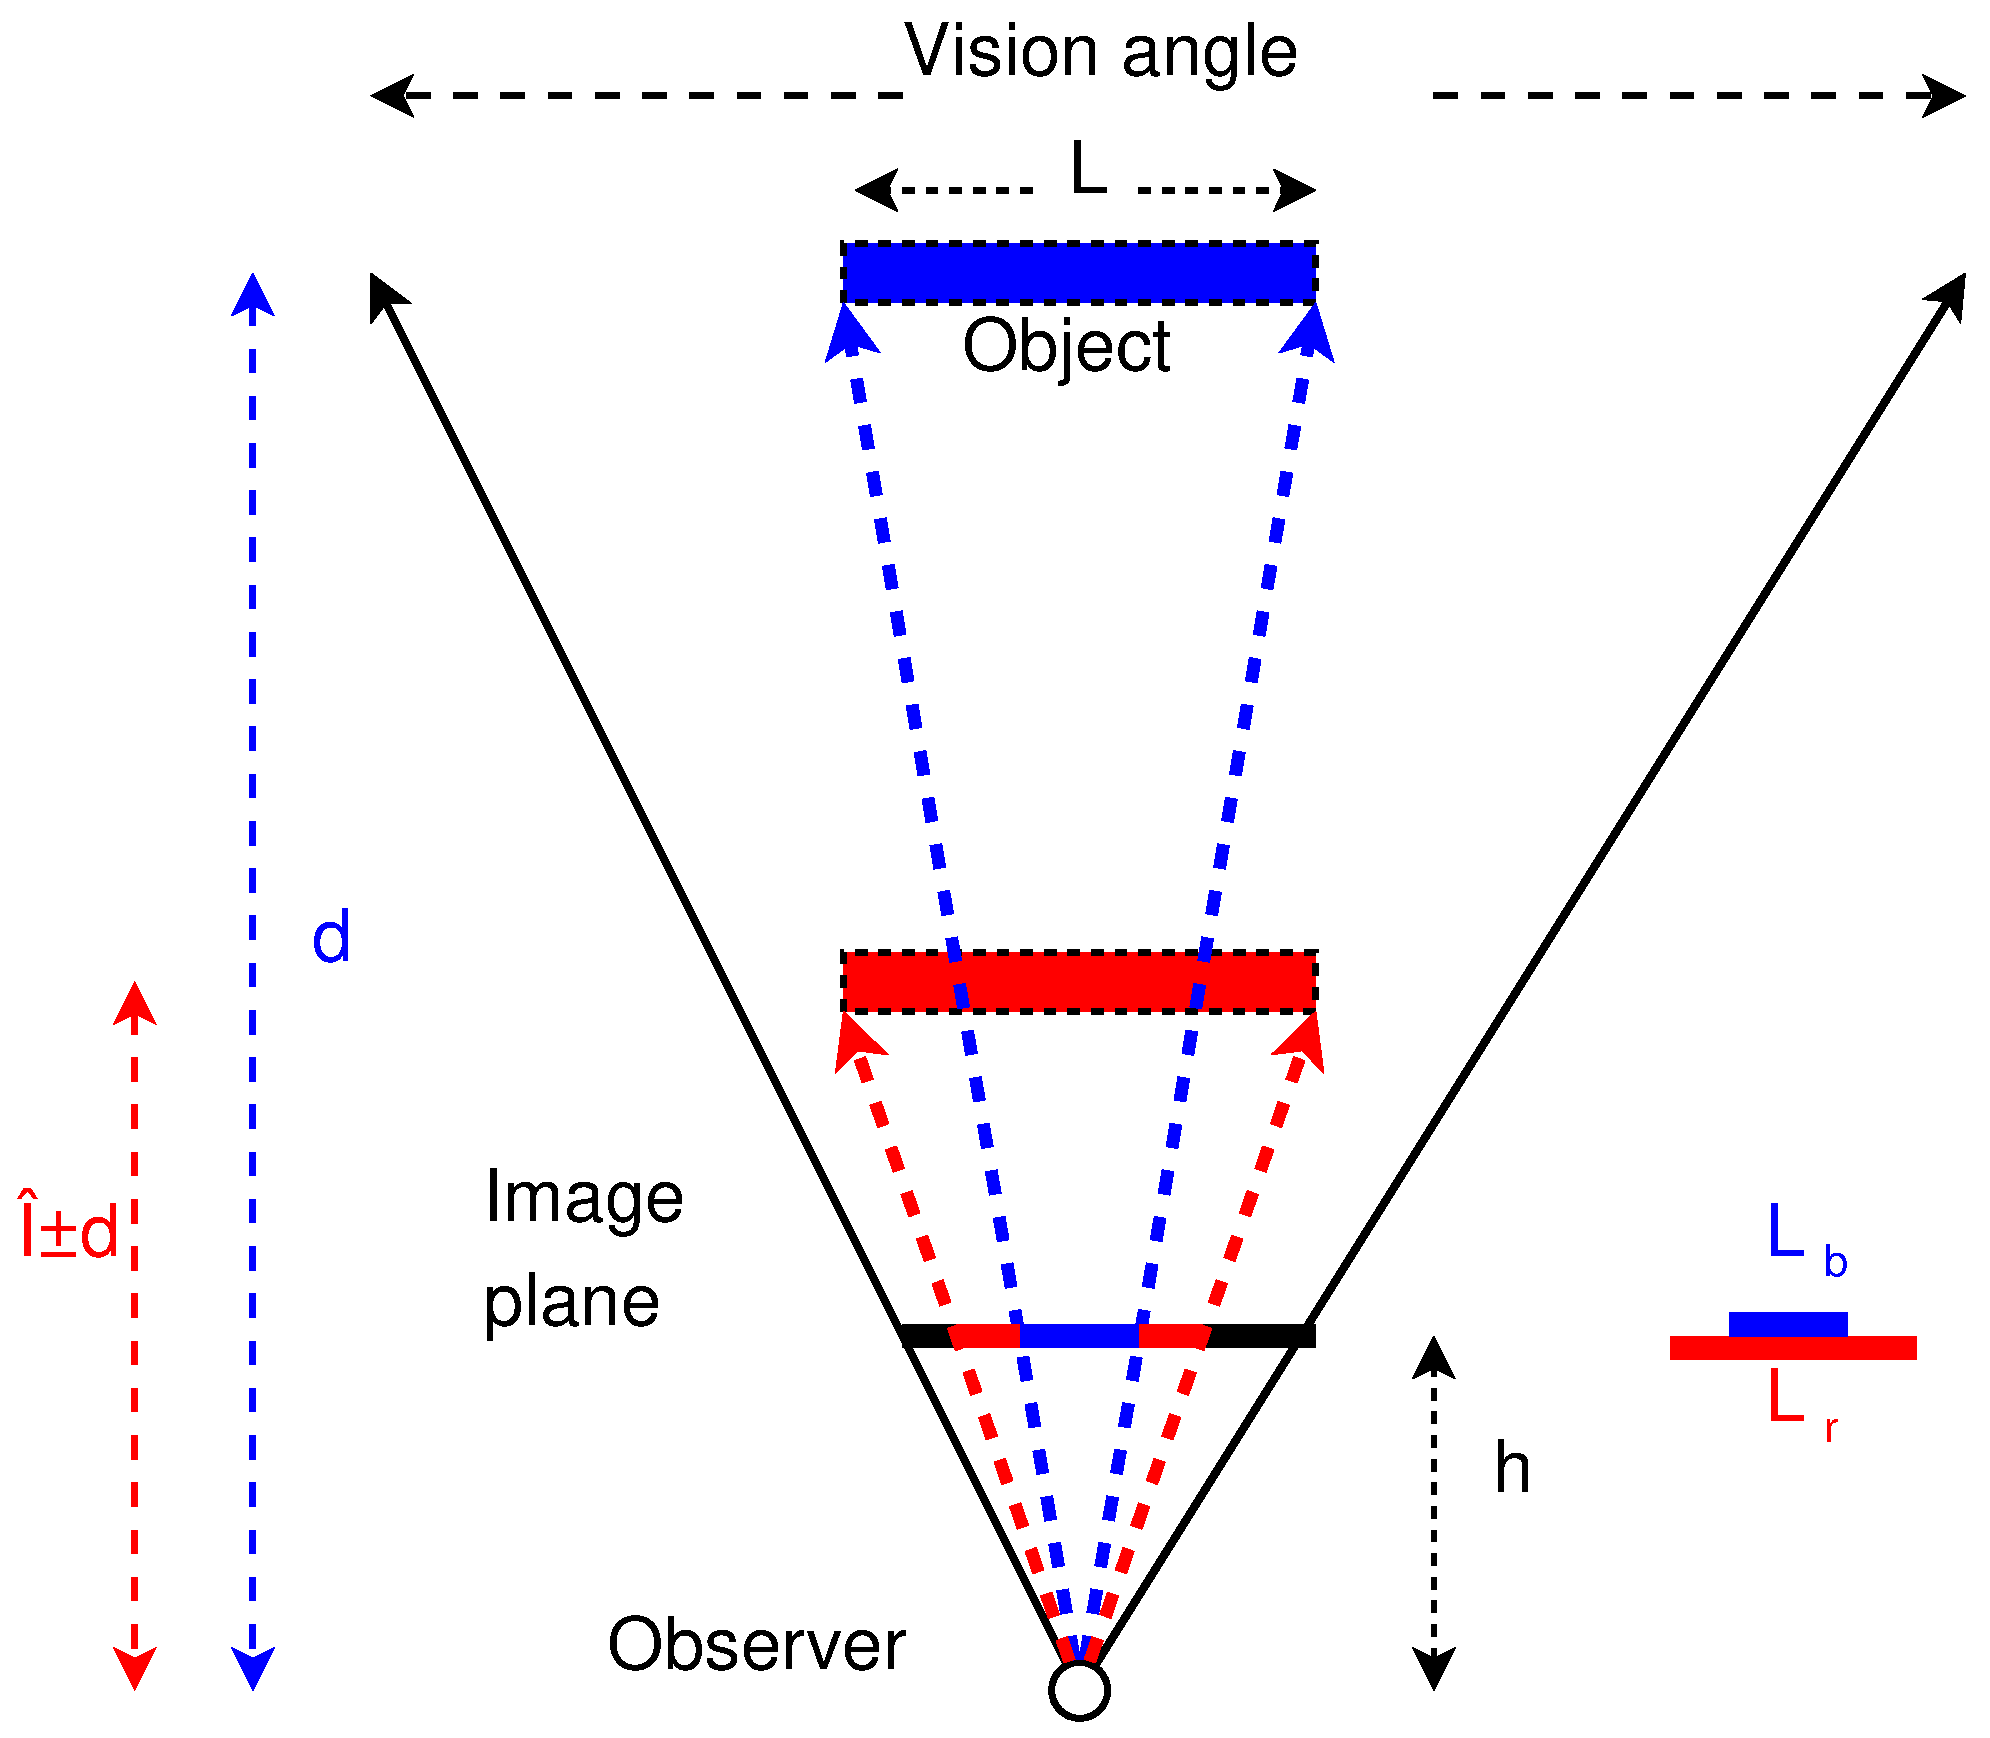
\includegraphics[width=.7\columnwidth]{images/Diagrama3.eps}
  \caption{ Acompanhamento do objeto em camadas.}
  \label{fig:multiscale3d}
\end{figure}

A fig. \ref{fig:multiscale3d} mostra o objeto em diferentes posições, 
$d$ e $\alpha d$, respectivamente em azul e vermelho.
O plano da imagem é definida pela distância $h$ do observador. As projeções dos objetos,
azul e vermelho, são representados por $L_b$ e$L_r$, respectivamente. Analisando a forma
triangular, é possível notar que $\frac{h}{d}=\frac{L_b}{L}$ e $\frac{h}{\alpha d}=\frac{L_r}{L}$, logo 
$L_b/\alpha= L_r$. 
Partindo do ponto de vista do observador, quando o objeto estava localizado na distância $d$ no tempo
$t_0$ e moveu-se para a distância $\alpha d$ no tempo $t_1$, o seu tamanho no plano da imagem 
foi alterado por um fator de 1/$\alpha$, e consequentemente, a área foi alterada por um fator 1/$\alpha^2$.

O critério de busca dos objetos usa valores discretos de $\alpha$, portanto o algoritmo busca o objeto
mais próximo com $\alpha<1$ e o mais distante com $\alpha>1$.



\subsubsection{Fator de aproximação - Velocidade Relativa}

O fator de aproximação é um número adimensional que relaciona a taxa de 
aproximação de um objeto em relação ao seu observador.
O fator é determinado pela equação (\ref{eq:relarea}),

\begin{equation}\label{eq:relarea}
f_a \equiv \alpha^2 \equiv \frac{Area_r}{Area_f} 
\end{equation}

Onde $f_a$ e $\alpha$ são definidos como um fator de área e de aproximação,
respectivamente; $Area_r$ é a área do $ROI$ e $Area_f$ é a área da região analisada
do último frame.

Conhecendo $\alpha$, se considerado que o objeto estava a uma distância $d_0$, então
sua próxima distância será $\alpha d_0$ (ou $\sqrt{f_a} d_0$). Assim, cada $i-ésimo$ imagem
terá o seu próprio $\alpha_i$ valor, onde $d_i=\alpha_i d_0$.

O fator de aproximação, $\alpha_i$, tem dois significados: se o fator de aproximação cresce rapidamente 
significa que o objeto está se afastando e se o fator decresce o objeto está se aproximando.

A velocidade relativa é definida pela equação da cinemática em física:

\begin{equation}
 v_i = \frac{\Delta s}{\Delta t}= \frac{s_i-s_{i-1}}{\Delta t}.
\end{equation}

Onde o vetor $v_i$ representa a velocidade relativa à $i-ésimo$ imagem, $s_i=(x_i,y_i,d_i)$ é a posição que
foi definida pela busca na $i-ésimo$ imagem e $\Delta t$ é o intervalo de tempo entre a análise das duas imagens.
Adicionalmente, o fator da velocidade de aproximação, $v^d_i$, é o número escalar o qual representa a componente
responsável pela profundida no vetor $v_i$.

O cálculo do valor $v^d_i$ se modifica, pois depende da distância entre a câmera e o objeto. No instante $i-ésimo$,
a distância será referenciada como $d_0$, sendo definida como valor 1.

\begin{comment}

\subsection{RENEW ROI CRITERION}
%Diagrama2
The $ROI$ is an important element in the algorithm, therefore it will be used
as pattern to find a match of tracked target at the current image. 
The  question in this case is to know the best moment to refresh the $ROI$
with a new perspective of target. 
Here, we establish the criterion that; when the comparison of images return 
a $PCC$ value lower than $0.925$ and greater than $0.8$, then the $ROI$ is changed with the current 
analyzed region and a new position of $ROI$ is with $(x_i,y_i,d_i)$. 
Thus, it was adopted as $0.8$ the lower limit to a match case\cite{Eugene},
see Fig. \ref{fig:newroicri}. Values less than $0.8$ causes a  lost target alert.
Finally, it is important to note that if the $ROI$ is changed, the new $ROI$ is 
the real size of the analyzed region and not with the rescaled version used
in the calculus of the $PCC$.


\begin{figure}[H]
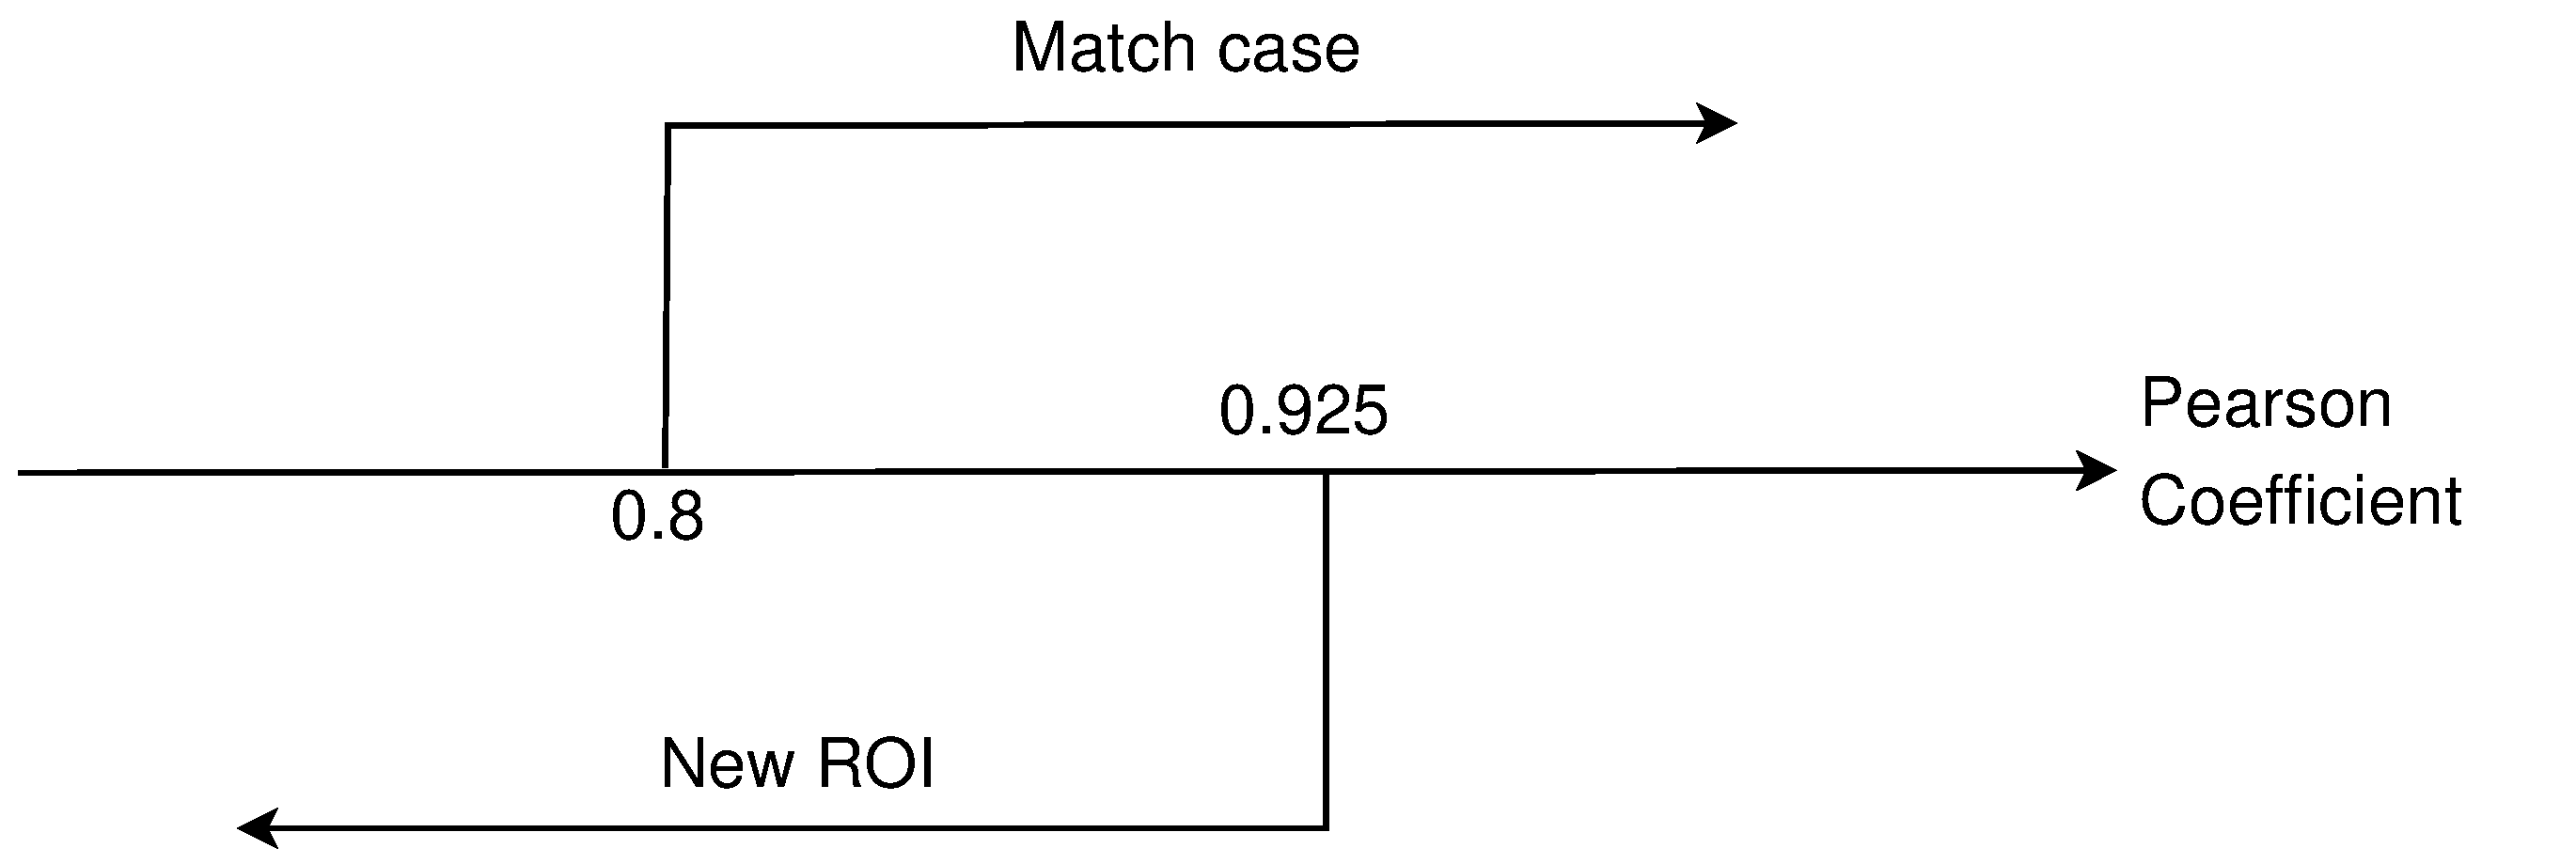
\includegraphics[width=\columnwidth]{images/figure3.eps}
\caption{When the comparison is greater than $0.8$, including numbers bigger than 
$0.925$, it means that the target was matched. But if two regions are compared 
and the $PCC$ is less than $0.925$ and greater than $0.8$, 
then the $ROI$ changes to the current analyzed region.}
\label{fig:newroicri}
\end{figure}

The Algorithm \ref{alg:newroi} shows the criteria described in the
Fig. \ref{fig:newroicri}; the $renew\_roi\_criteria()$ function, explained here,
it is used by the Algorithm \ref{alg:system} of Fig. \ref{fig:system}.

\begin{algorithm}
 \KwData{Initial $ROI$, your position $P_0$, the current matched analysis region ($AR$), your position $P$ and the correlation $r$ between them. }
 \KwResult{The new $ROI$, your position and a status variable, $Found$. }

    $NEWP_0 \leftarrow  P_0$ \;
    $NEWROI \leftarrow  ROI$ \;
    
    \eIf{$0.8 \leq r$}
    {
      $Found \leftarrow True$\;
        message ``target found''\;
        \eIf{$r \leq 0.925$}
        {
            $NEWROI \leftarrow  AR$\;
            $NEWP_0 \leftarrow  P$\;
        }
    }
    {
      message ``target lost''\;
      $Found \leftarrow False$\;
    }
\Return  $\{NEWROI,~NEWP_0,~FOUND\}$\;
\label{alg:newroi}
\caption{$renew\_roi\_criteria(ROI,P_0,AR,P,r)$ function.}
\end{algorithm}
%The system needs to have a high level of reliability, so that the lower limit adopted 
%contributes to an operation with minimum of mistakes.

\end{comment}

%%%%%%%%%%%%%%%%%%%%%%%%%%portugues%%%%%%%%%%%%%%%%%%%%%%%%%%%%%%%%%%%%%%%%%%%%%%%%%%%%%%%



\subsection{Critério para um novo ROI}

O $ROI$ é um importante elemento dentro algoritmo, pois ele é a referência do
atual estado do objeto que será comparado com as imagens posteriores.
O critério para atualizar o $ROI$ é determinado a partir da correlação 
entre as imagens, sendo assim, se o valor da comparação estiver entre $0,925$ 
e $0,8$ o $ROI$ será atualizado com uma nova posição $(x_i,y_i,d_i)$.

Deste modo, foi adotado que o limite inferior é de 0,8 \cite{Eugene}. Valores
de comparação abaixo deste, o objeto é tido como perdido, como mostrado na figura
\ref{fig:newroicri}.
Nota-se que o $ROI$ é atualizado para uma escala igual a anterior ou modificada,
dependendo do valor da comparação dada pelo $PCC$.


\begin{figure}[H]
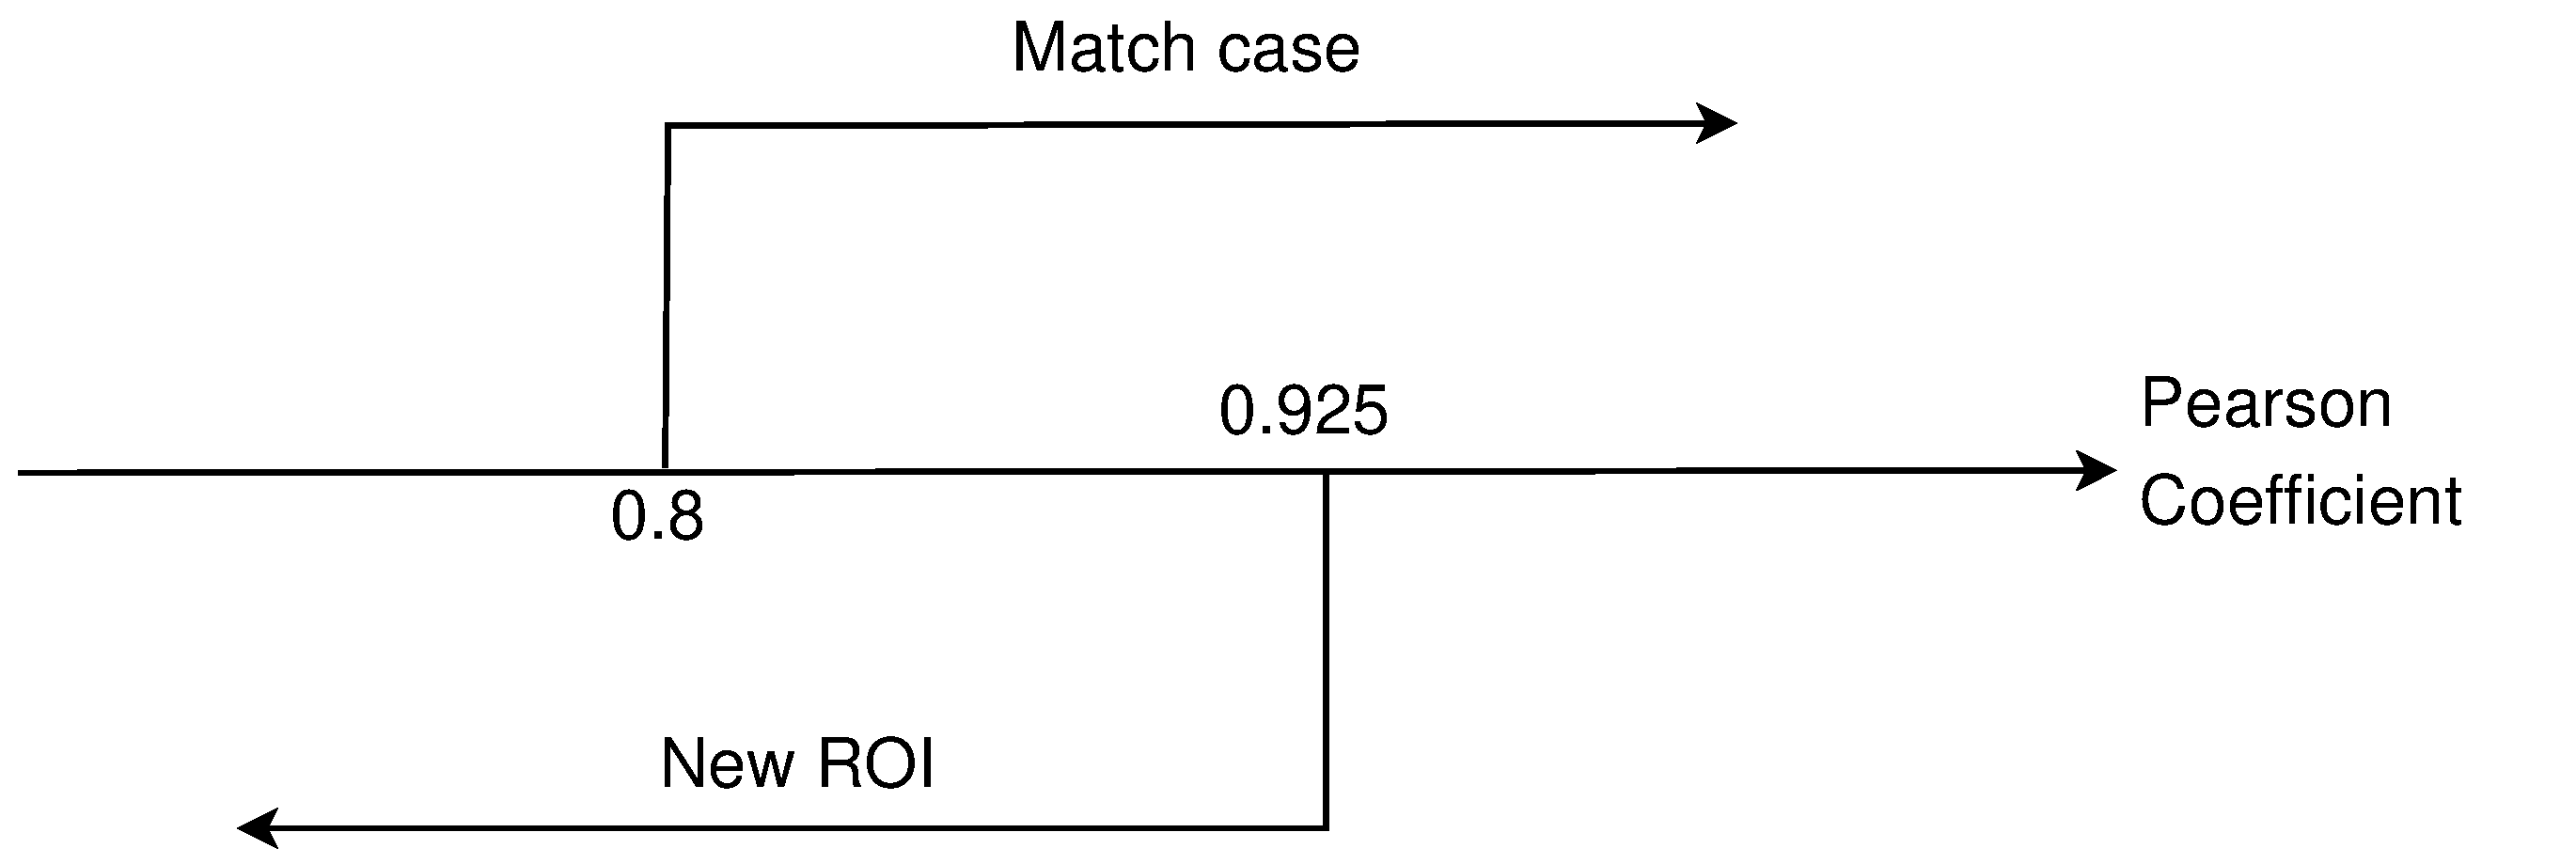
\includegraphics[width=\columnwidth]{images/figure3.eps}
\caption{Quando a comparação é maior que $0,8$, incluindo número maiores que $0,925$, significa que o objeto foi encontrado,
se o PCC é menor que $0,925$ a imagem é tida como perdida e se o coeficiente for maior que $0,8$, então o ROI é atualizado pela imagem de 
maior correlação.}
\label{fig:newroicri}
\end{figure}

O algoritmo \ref{alg:newroi} apresenta o critério descrito na figura \ref{fig:newroicri};
A função $renew\_roi\_criteria()$ explicada é usada pelo algoritmo \ref{alg:system} da figura \ref{fig:system}


\begin{algorithm}
 \KwData{$ROI$ inicial, posição $P_0$, região de busca do frame atual ($AR$), posição $P$ e a correlação $r$ entre eles. }
 \KwResult{O $ROI$ atualizado, posição e seu status, $Found$. }

    $NEWP_0 \leftarrow  P_0$ \;
    $NEWROI \leftarrow  ROI$ \;
    
    \eIf{$0.8 \leq r$}
    {
      $Found \leftarrow True$\;
        message ``target found''\;
        \If{$r \leq 0.925$}
        {
            $NEWROI \leftarrow  AR$\;
            $NEWP_0 \leftarrow  P$\;
        }
    }
    {
      message ``target lost''\;
      $Found \leftarrow False$\;
    }
\Return  $\{NEWROI,~NEWP_0,~FOUND\}$\;
\label{alg:newroi}
\caption{$renew\_roi\_criteria(ROI,P_0,AR,P,r)$ function.}
\end{algorithm}
%The system needs to have a high level of reliability, so that the lower limit adopted 
%contributes to an operation with minimum of mistakes.


% descrição do sistemA
\section{RESULTADOS EXPERIMENTAIS}
\begin{comment}


The followed informations introduce the results of two different tests 
using POV-Ray.

In the first test, Fig. \ref{fig:imgpapercerta}, 
the algorithm makes the tracking of an object through 14 images in sequence with 
a horizontal displacement to the camera.

\begin{figure}[H]
\centering
  \subfloat[]{\label{fig:imgpapercertaa} 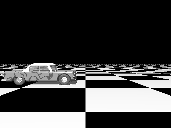
\includegraphics[width=.48\columnwidth]{images/results_2D.png}}
  \subfloat[]{\label{fig:imgpapercertab} 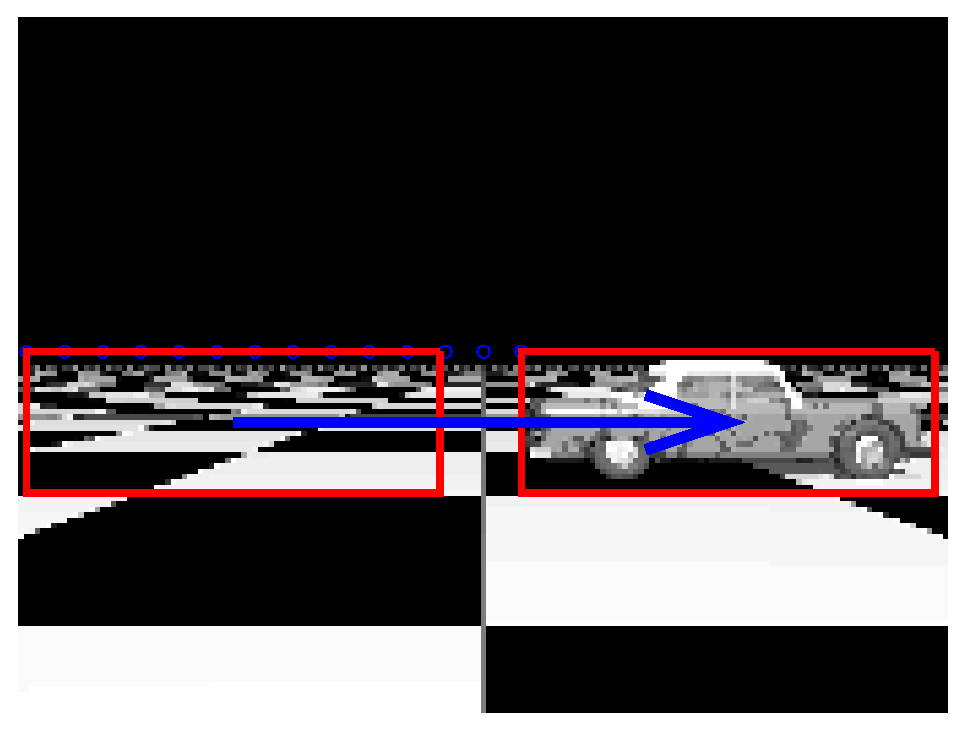
\includegraphics[width=.48\columnwidth]{images/results_2D.eps}}
  \caption{The image in (a) represents the target in its initial position 
   and the image (b) shows the vehicle in its final position.}
  \label{fig:imgpapercerta}
\end{figure}

The initial position of target is in the image (a) and the final position in (b), 
where a vector (in blue) illustrates the resulting trace.
We can observe that there is a small bend in the image 
and it generates a slight change of object perspective. 
The update of the $ROI$ is frequently done, which involves seeing a slight change in area.
The difference between the initial and final values of the departure factor may 
be considered constant, and the value is 1. It means that image doesn't approach to the camera
%as shown in Fig. \ref{fig:res_graph1}.

%\begin{figure}[H]
%\centering
%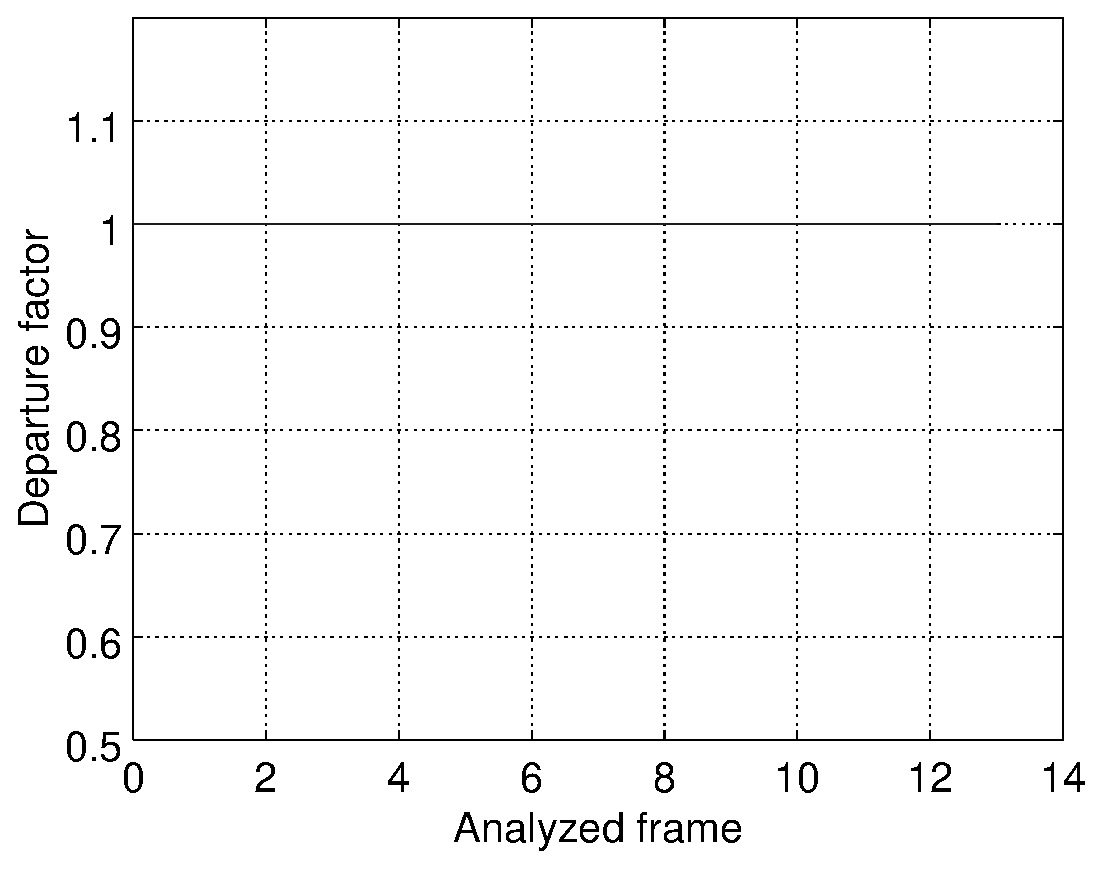
\includegraphics[width=0.8\columnwidth]{images/results2D_graph.eps}
%\caption{Departure factor for each frame in the test 1.}
%\label{fig:res_graph1}
%\end{figure}

%Fig. \ref{fig:res_graph1v} shows 
The value of the velocity of departure factor is $d_0=1$ and $\Delta t=1$. 
It demonstrates that the variation
of the departure factor is 0 when compared with 1. 
It has departure factor (velocity) of $0$. Target is at same distance 
during 14 frames in relation camera.
.
%\begin{figure}[H]
%\centering
%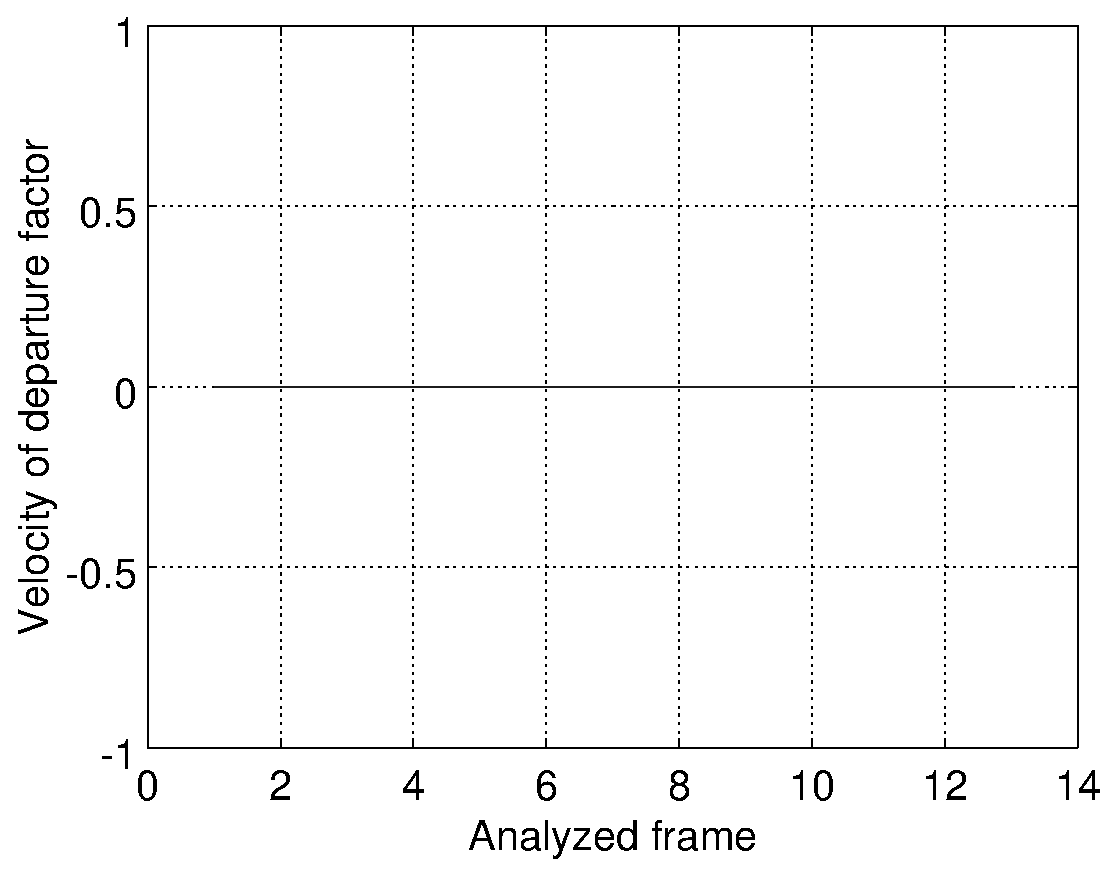
\includegraphics[width=0.8\columnwidth]{images/results2D_graphv.eps}
%\caption{Velocity of departure factor for each frame in the test 1.}
%\label{fig:res_graph1v}
%\end{figure}

In test 1, we can observed the movement in axis X and rotation of target, the last one causes change of ROI more frequent
because PCC generates a value below of threshold defined in Fig. \ref{fig:newroicri}.
The high changes of ROI for rotation of target can be showed by bubbles in the superior part of ROI in Fig. 
\ref{fig:imgpapercerta} (b).

\end{comment}

%%%%%%%%%%%%%%%%%%%%%%%%%%%%%%%%%%%%%%%%%%portugues%%%%%%%%%%%%%%%%%%%%%%%%%%%%%%%%%%%%%%%%%%%%%%%


O resultados a seguir foram obtidos nos testes usando o simulador POV-Ray.

No primeiro teste, o algoritmo acompanha o objeto que está em um movimento horizontal em relação a câmera
pelas sequência das 14 imagens, como mostrado na figura \ref{fig:imgpapercerta}

\begin{figure}[H]
\centering
  \subfloat[]{\label{fig:imgpapercertaa} 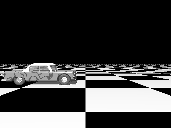
\includegraphics[width=.48\columnwidth]{images/results_2D.png}}
  \subfloat[]{\label{fig:imgpapercertab} 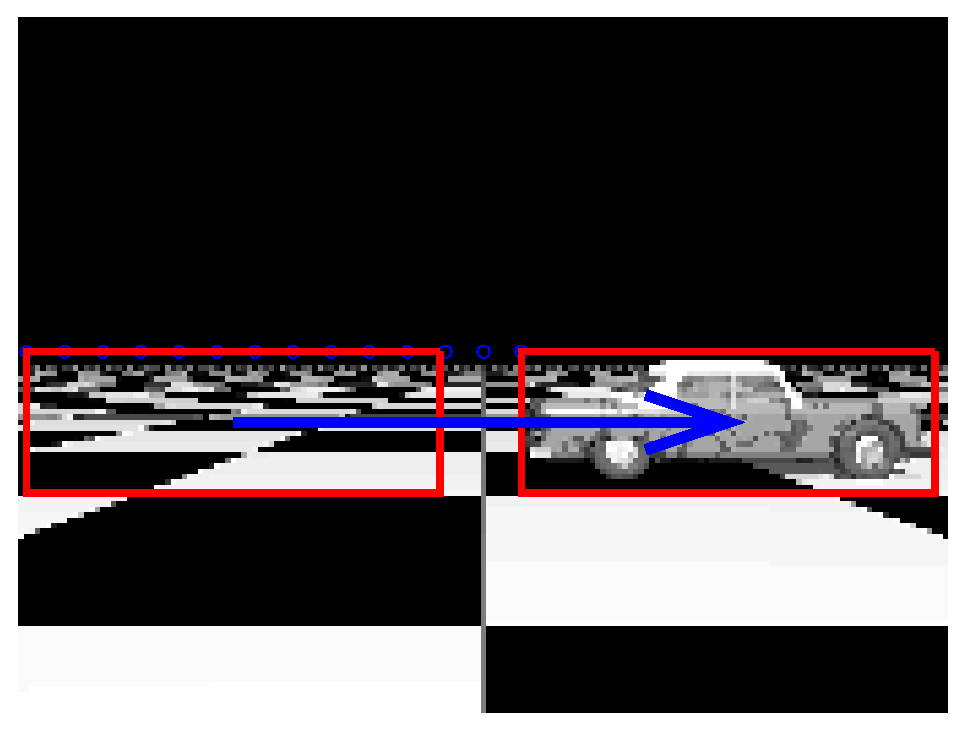
\includegraphics[width=.48\columnwidth]{images/results_2D.eps}}
  \caption{A imagem (a) representa o objeto em sua posição inicial  
   e a imagem (b) mostra na sua posição final.}
  \label{fig:imgpapercerta}
\end{figure}

A posiçao inicial do objeto está na imagem (a) e a final na (b). De modo que o
vetor em azul é o resultado da busca feita, ligando a posição inicial com a final.
Nota-se neste testa, também, uma pequena curvatura na imagem o que ocasiona uma mudança
na perspectiva do objeto, resultando em uma mudança frequente do $ROI$.
A diferença entre o valor inicial e final do fator de aproximação é considerado constante
e igual 1, pois o objeto não se aproxima da câmera.

Neste teste, a velocidade do fator de aproximação é zero, pois não há aproximação e nem
afastamento do objeto em relação a câmera, sendo $d_0=1$ e $\Delta t=1$.

No teste 1, observa-se uma modificação frequente no ROI e isso ocorre porque as imagens 
tem uma semelhança menor do que a definida, como mostrando na figura \ref{fig:newroicri}. 
Na figura\ref{fig:imgpapercerta} (b), é possível identificar a quantidade de atualizações feitas no $ROI$,
 pois são indicadas com bolas no canto superior esquerdo da imagem.



\begin{comment}
 In the second test, we prove the functionality of the algorithm in three dimensions. 

The algorithm compares the images and calculates the departure factor 
based on area of ROI. Fig. \ref{fig:target} demonstrates the 
tracking of $40$ images from initial position to the final position of the target, 
highlighted with red boxes;
the vector in blue describes the movement of the target. 

\begin{figure}[H]
\centering
  \subfloat[]{\label{fig:targeinit} 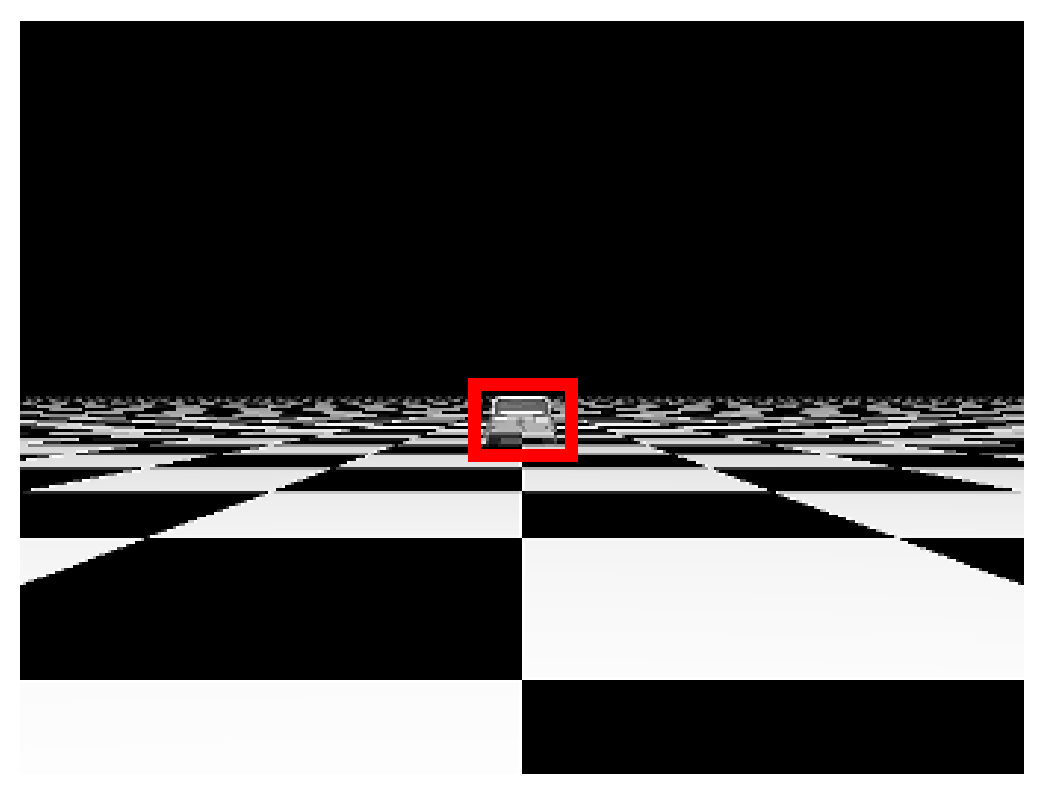
\includegraphics[width=.48\columnwidth]{images/figurea.eps}}
  \subfloat[]{\label{fig:targeend} 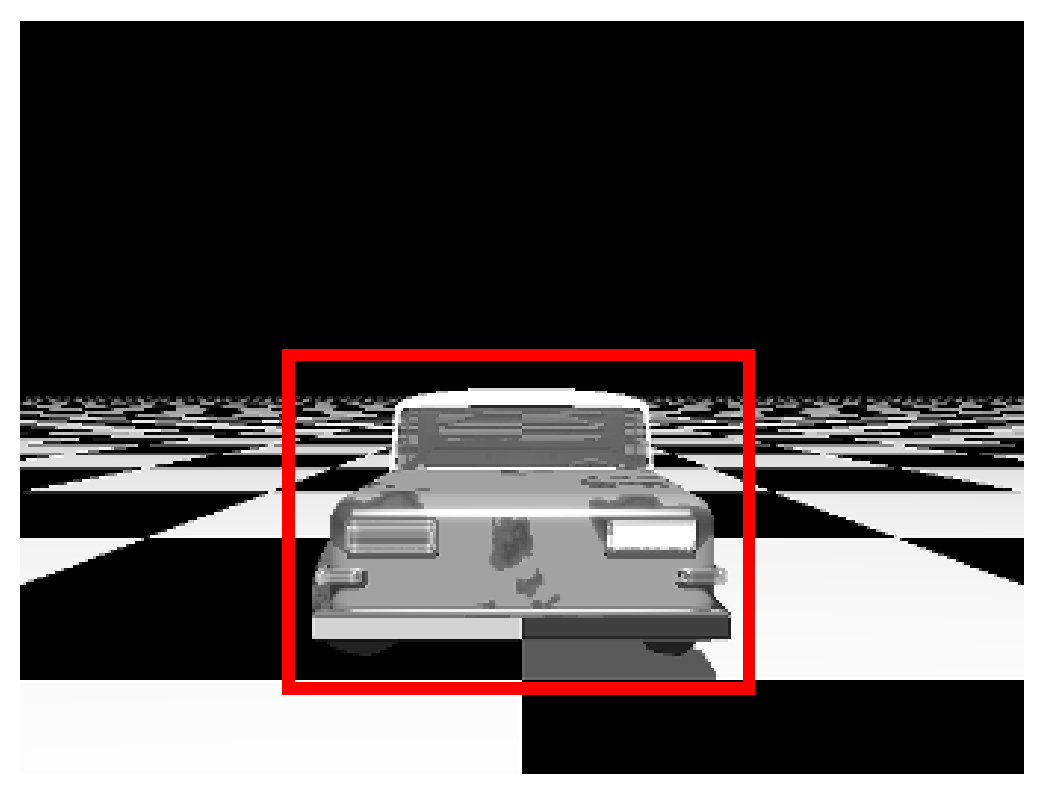
\includegraphics[width=.48\columnwidth]{images/figureb.eps}}
  \caption{The target in (a) is the initial position and its area is smaller than the target in (b), 
  which represents the final position. The factor is dividing both areas.}
  \label{fig:target}
\end{figure}

In Fig. \ref{fig:target}, we can observe an increase in ROI, and 
its influence to the departure factor is shown in Fig. \ref{fig:res_grapha_b}.

\begin{figure}[H]
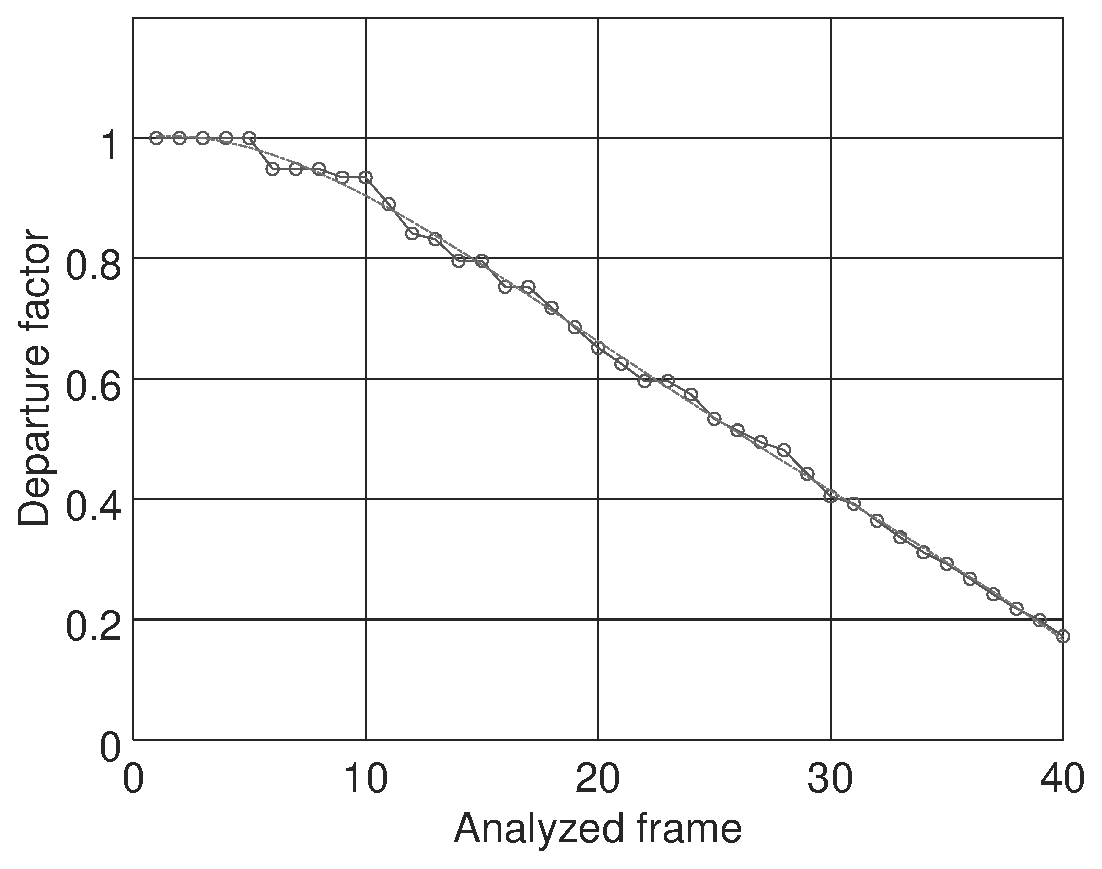
\includegraphics[width=\columnwidth]{images/grapha_b.eps}
\caption{Departure factor for each frame in the test 2.}
\label{fig:res_grapha_b}
\end{figure}

The Fig. \ref{fig:res_grapha_b} shows the departure factor in each frame
of test 2 (see the line with circles), additionally It is showed a polynomial
fitting of departure factor using a polynomial of order 4 (see the line with dots),
finally It is showed the real route of target normalized to $1.0$ for the maximum distance
(see the line with squares), as can be seen the target is approaching with a constant speed. 
If we interpret this value as the position in each sample time, 
then the departure factor describes the relative target position.
In the first image the analyzed target is at a distance $d_0$ 
and in the last image the target is at a distance of $17.18\%$ of $d_0$.
The departure distance decreases in discrete steps because the departure
factor is selected in discrete steps, if the target is
between two consecutive analysis layers (scales), the algorithm
approximates the target to the nearest layer.



The Table \ref{tab:tab1} represents the bank of images used for test 2, totally 40 images generated by POV-Ray.
The number of analyzed frames are in the first column of table, in the second column are the real distances 
between camera and target.
The percentage proportion of real distances are in third column. For example, 
the target in first frame is to $23.5$ meters from camera and it is considered the $100$\% of distance,
by other side, in the frame $40$ the target is to $4$ meters 
from camera and is $17,02$\% in relation of first frame. Next column, fourth column, 
we have the results of algorithm (departure factor), in the percentage form. 
%Note in first frame, target is $100$\% of distance and the last frame is at $17,18$\% of distance in relation of first frame.
Finally, the last column represents the error between percentage real distance and the departure factor. 
As can be seen, the error is diminishing when target is close (around 5 meters), it means that the algorithm has more precision 
when image of target is bigger because there are more information in ROI. It is a consequence of CCP, 
because in small ROI each pixel charge much information in comparative method. On other hand, if ROI is bigger,
the information is diluted around pixels; thus, the algorithm has more data to compare.
Another reason is that in the last frames $1$ pixel of target
represents a less distance in meters that $1$ pixel in the target of the first frames; consequently, the error 
of a quantity $x$ of pixels represents a less quantity of error meters in the analysis of last frames.

\begin{table}[H]
\setlength{\tabcolsep}{1 pt} 
\caption{Table of comparative results}
\begin{tabular}{lllll}
Frames & Real Dist. (m) & Real Dist. (\%) & Dep. factor (\%) & Relative error (\%)\\
1 & 23.5 & 100.0 & 100.0 & 0.0 \\
10 & 19.0 & 80.85 & 93.46 & 15.60 \\
20 & 14.0 & 59.57 & 65.16 & 9.37 \\
30 & 9.0 & 38.30 & 40.46 & 5.65 \\
40 & 4.0 & 17.02 & 17.18 & 0.93
\end{tabular}
\label{tab:tab1}
\end{table}

The Fig. \ref{fig:res_grapha_bv} shows the velocities of the data showed in the 
Fig. \ref{fig:res_grapha_b}  calculated to $d_0=1$ and $\Delta t=1$. 
Thus, it is showed the velocity of departure factor (see the line with circles), 
additionally It is showed the velocity of the polynomial
fitting of departure factor (see the line with dots) and
finally It is showed the velocity of the normalized real route
(see the line with squares), being it a constant.
The velocities were calculated using the discrete-time derivate.
The values of the velocities are negatives, which indicates that the
target is approaching towards the observer. As can be seen,
the velocity of the departure factor don't have a monotone behavior 
because that the curve of the departure factor has a many discrete changes; thus,
It is important to use the polynomial fitting curve
to calculate the velocity, because this curve represents
very close the behavior of the velocity of the normalized real route.

\begin{figure}[!hbt]
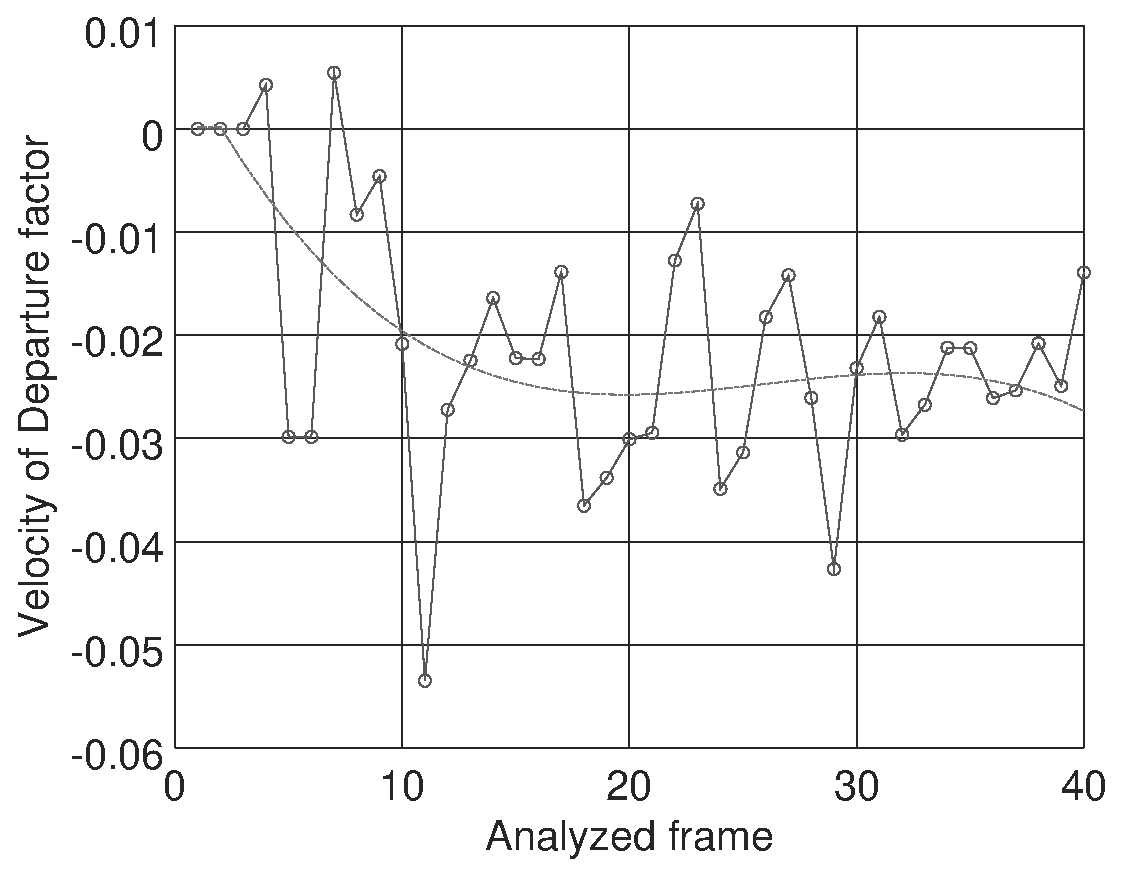
\includegraphics[width=\columnwidth]{images/graphvelocity.eps}
\caption{Velocity of departure factor for each frame in test 2.}
\label{fig:res_grapha_bv}
\end{figure}

\end{comment}


%%%%%%%%%%%%%%%%%%%%%%%%%%%%%%%%%%portugues%%%%%%%%%%%%%%%%%%%%%%%%%%%%%%%%%%%%%%%%%%%%%%%%
A funcionalidade do algoritmo para um caso em $3D$ é verificada no segundo teste;
nele, similar ao primeiro teste, o algoritmo compara um conjunto de imagens 
e calcula o fator de aproximação; porém, neste caso, o objeto de interesse tem um movimento
relativo em direção ao observador. A Figura \ref{fig:target} representa o 
rastreamento  do objeto de interesse em um fluxo de 40 imagens sequenciais. Os retângulos vermelhos
são as posições das regiões de análise inicial e final.

\begin{figure}[H]
\centering
  \subfloat[]{\label{fig:targeinit} 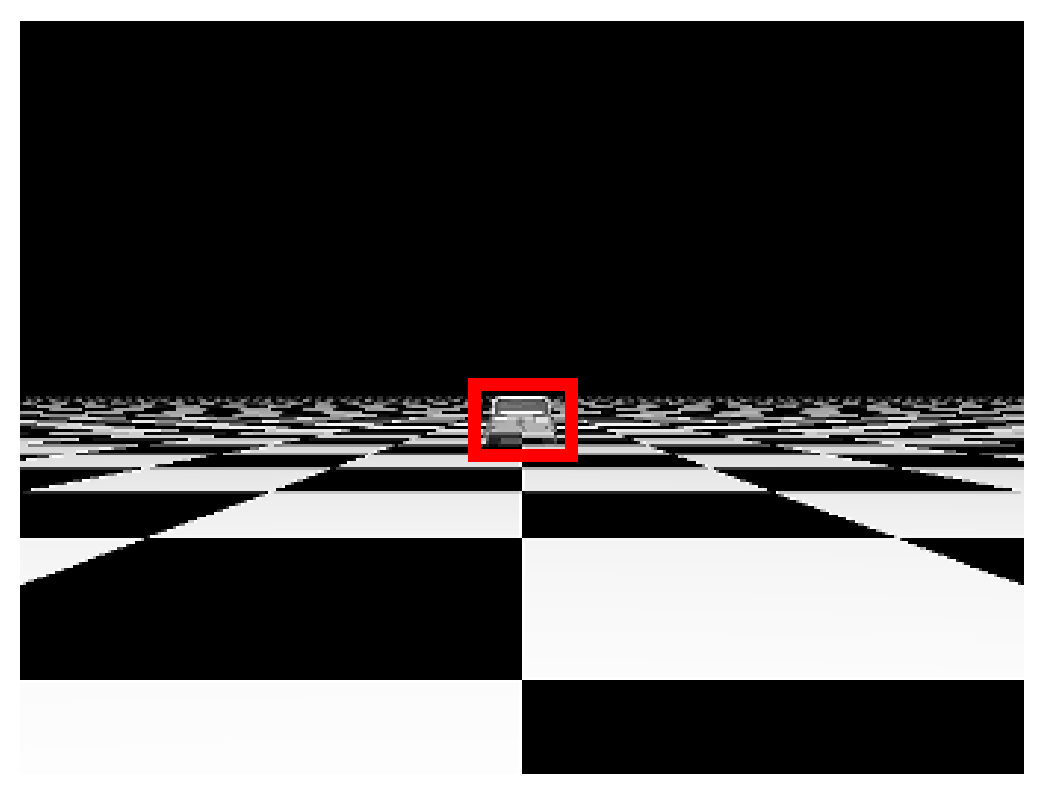
\includegraphics[width=.48\columnwidth]{images/figurea.eps}}
  \subfloat[]{\label{fig:targeend} 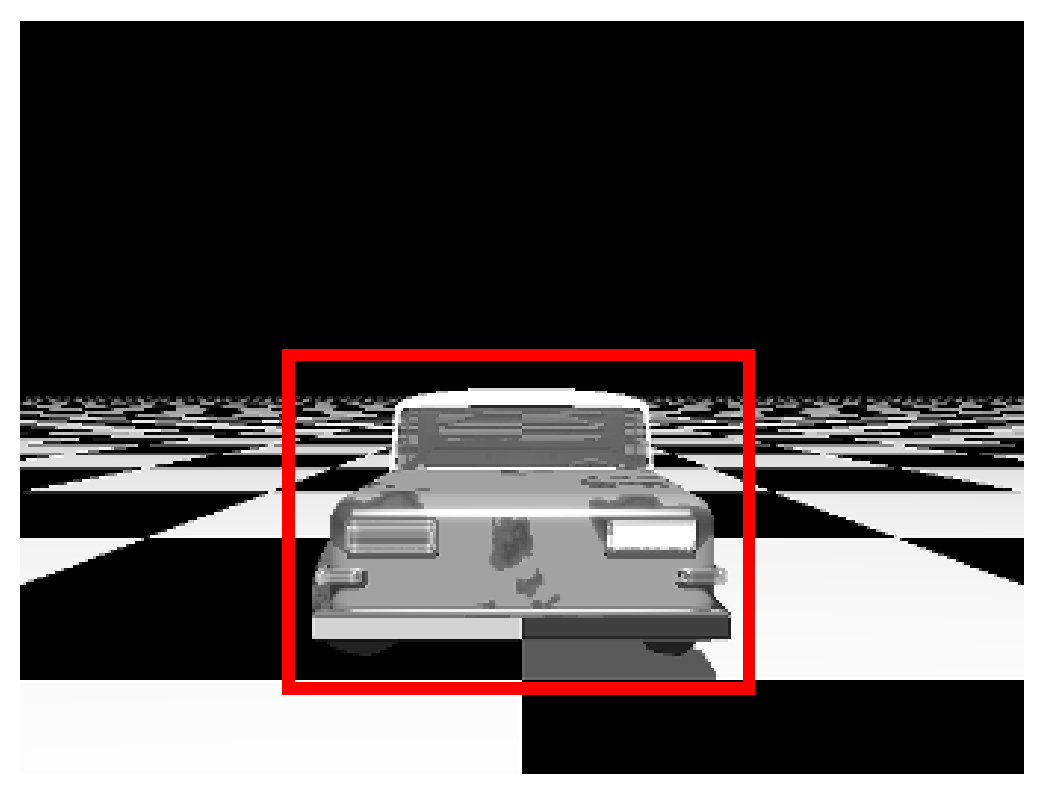
\includegraphics[width=.48\columnwidth]{images/figureb.eps}}
  \caption{O Objeto de interesse em (a) está na posição inicial com área menor que em (b), 
  a posição final.}
  \label{fig:target}
\end{figure}

Na Figura \ref{fig:target}, observa-se um crescimento na $ROI$ e, por
consequência, uma modificação do fator de aproximação $\beta$ relativo a $d_0$.
A Figura \ref{fig:res_grapha_b} apresenta o fator $\beta$ para cada uma das imagens 
do teste 2 (representado na linha com círculos).
Além disso, um ajuste polinomial deste fator a partir de um polinômio de ordem 4 é apresentado na linha pontilhada.
Finalmente, na linha com quadrados, é apresentada a distância normalizada entre o objeto de interesse e o observador,
de modo que a distância inicial $d_0=1.0$.
Como pode ser visto, o alvo está se aproximando com uma velocidade constante.
\begin{figure}[H]
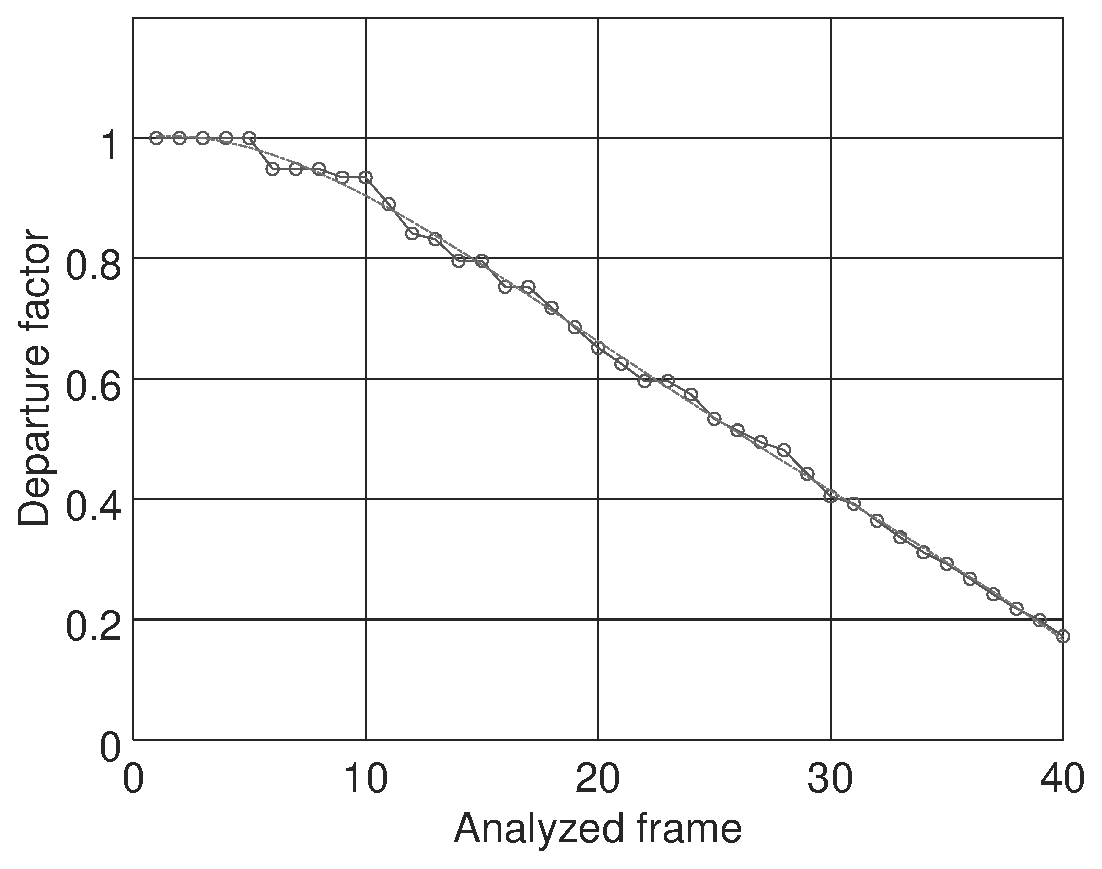
\includegraphics[width=\columnwidth]{images/grapha_b.eps}
\caption{O fator de aproximação $\beta$ relativo a $d_0$, para cada uma das imagens do teste 2.}
\label{fig:res_grapha_b}
\end{figure}


A tabela \ref{tab:tab1} descreve o resultado da análise do banco 
de imagens usado no teste 2, sendo um total de 40 imagens geradas
pelo programa de simulação POV-Ray.
\begin{table}[H]
\setlength{\tabcolsep}{1 pt} 
\caption{Tabela de resultados}
\begin{tabular}{l|l|l|l|l}
Imagem & Real Dist.(m) & Real Dist.(\%) & Fator de aprox.(\%) & Erro relativo(\%)\\ \hline  \hline
1 & 23.5 & 100.0 & 100.0 & 0.0 \\ \hline
10 & 19.0 & 80.85 & 93.46 & 15.60 \\ \hline
20 & 14.0 & 59.57 & 65.16 & 9.37 \\ \hline
30 & 9.0 & 38.30 & 40.46 & 5.65 \\ \hline
40 & 4.0 & 17.02 & 17.18 & 0.93 \\ \hline
\end{tabular}
\label{tab:tab1}
\end{table}
A primeira coluna representa o número da imagem analisada, e por uma questão de espaço, foram selecionados 
os resultados a cada 10 imagens; a segunda coluna contém a distância 
real em metros entre o objeto de interesse e o observador.
A porcentagem da distância real com $d_0$ está representada na terceira coluna. Por exemplo, o objeto na primeira imagem
está a $23.5$ metros da câmera, por outro lado, na imagem 40 o objeto está a
$4$ metros da câmera, apresentando uma distância de  $17,02$\% em relação a 
primeira imagem. Na quarta coluna estão os resultados do algoritmo (fator
de aproximação $\beta$ relativo a $d_0$) em porcentagem. Finalmente, a última coluna representa o erro 
entre a porcentagem da distância real e $\beta$.

Dado que é adotado um valor normalizado de $d_0=1,0$ como a posição do objeto de interesse na primeira 
imagem, então o fator de aproximação $\beta_i$ na imagem $I_i$ é 
numericamente igual a $d_i$, e descreve a posição relativa do objeto.
Assim, na primeira imagem o objeto analisado está a uma distância $d_0$
e na última imagem a uma distância $d_{40}=17.18\%d_0$.

É importante ressaltar que a aproximação do objeto à câmera é analisada de forma discreta, 
portanto, se o objeto
estiver entre duas camadas da análise, o algoritmo aproxima o resultado para
a camada mais próxima. Estas camadas são geradas pelo uso do fator $\alpha$
descrito no algoritmo \ref{alg:multires}. Outra consequência desta discretização
é a dificuldade de medir deslocamentos horizontais ou verticais, ou aumentos laterais da região de análise,
menores a $1$ pixel, de modo que quanto maior for a quantidade de pixels por
imagem analisada melhor será o desempenho do algoritmo para deslocamentos ou variações de área.

Um ponto a ser ressaltado é a diminuição do erro para distâncias próximas a 5 metros.  
Os resultados mostram que o algoritmo tem mais precisão conforme o objeto de interesse 
aumenta de área na imagem; pois este contém mais pixels (informação)
para os cálculos e, adicionalmente, cada pixel no objeto de interesse 
representa uma quantidade menor de metros na cena, de modo que
o erro em metros diminui.
Assim, no método de comparação ($CCP$), nota-se que quanto menor for a $ROI$ 
maior será o impacto do erro em cada pixel da imagem, 
e por consequência, menor precisão na descrição do objeto de interesse. 
Contudo, se o objeto de interesse cresce de tamanho na cena,
o método terá regiões de analise com mais informação (mais pixels), e menor porcentagem de metros do objeto por pixel,
o que leva a ter um erro em metros mais controlado, conforme pode se constatar nos testes realizados. 

A Figura \ref{fig:res_grapha_bv} apresenta a velocidade dos dados da 
Figura \ref{fig:res_grapha_b}, calculados para $d_0=1$ e $\Delta t=1$.
Assim, a velocidade do fator $\beta$ (linha com círculos) é ajustada por um polinômio
normalizado (linha pontilhada), segundo o percurso real do objeto (linha com quadrados).
A velocidade relativa do objeto foi calculada usando a derivada
discreta, sendo que os valores negativos indicam que o objeto está
em direção ao observador.

Para calcular a velocidade é necessário usar um ajuste polinomial devido 
as mudanças abruptas e erros causados pela discretização dos dados pelo fator $\beta$.
Assim, obtém-se uma descrição mais próxima da velocidade relativa do 
objeto de interesse.

\begin{figure}[H]
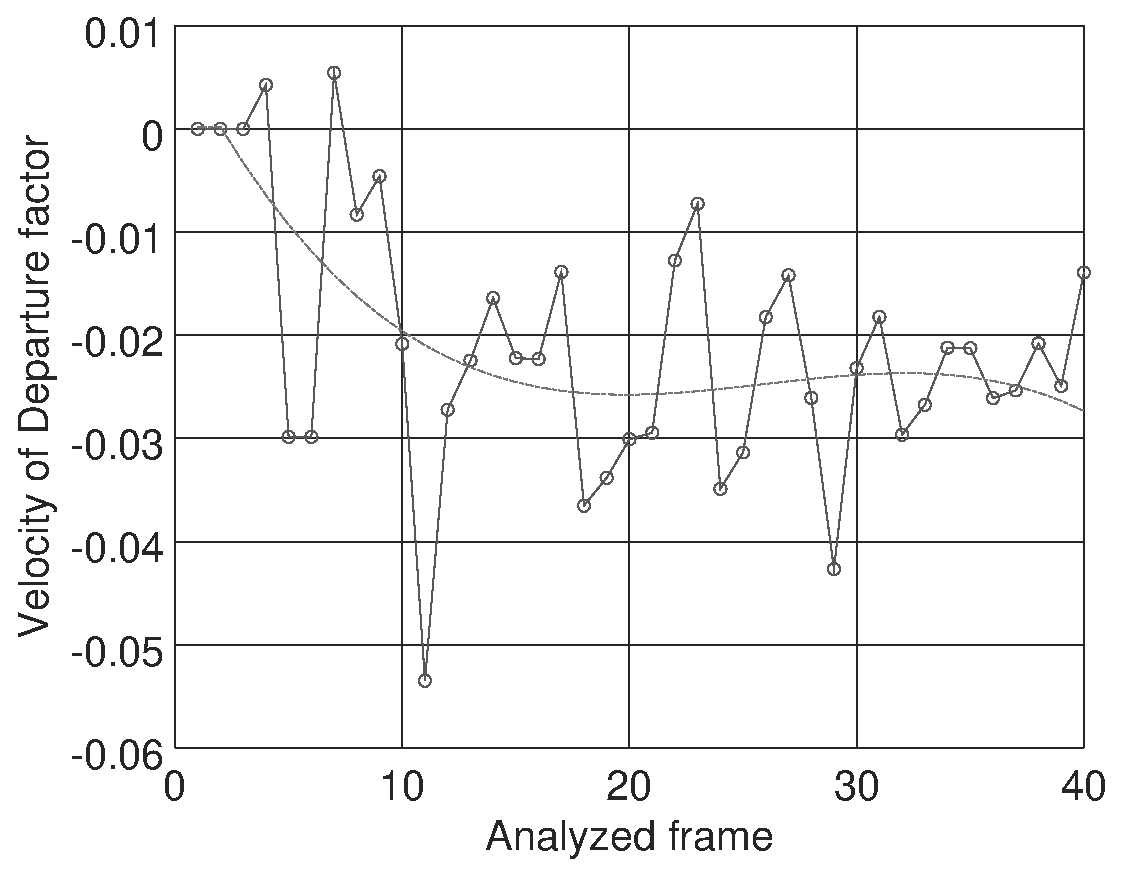
\includegraphics[width=\columnwidth]{images/graphvelocity.eps}
\caption{Velocidade das curvas normalizadas para cada um dos resultados obtidos no teste 2.}
\label{fig:res_grapha_bv}
\end{figure}

%testes com diferentes parametros
% tabelas e graficos



\section{CONCLUSÃO}
%From the presented examples,
it is possible to see that one application that uses the tracking
and the departure factor is related with risk of collision.
It is possible to estimate how of fast an object is departing,
and thus, if the  departure factor tends to zero or 
if the velocity of departure factor changes to lower negatives values every time, 
probably, there is a high risk of collision.

The $PIV$ technique has presented satisfactory results. 
Different kinds of information can be concluded, 
like: estimate collision using velocity of departure factor, 
tracking of objects in 2 or 3 dimensions and departure distance
relative to the first position of $ROI$. 
The simulations in both cases has given promissory results.

%\addtolength{\textheight}{-12cm}

%\section*{ACKNOWLEDGMENT}

%We want to thank to FAPEMIG, LMT and UFLA for support given to this research.
Project number associated to this research by FAPEMIG: PIDEG37-2015.

%FAPEMIG\\
%numero de bolsa\\
%numero de projeto\\
%numero de aluno


\begin{thebibliography}{99}
	\bibitem{Bastiaans} R. J. M. Bastiaans, Cross-correlation PIV; theory, implementation and accuracy. 
        Eindhoven: Technische Universiteit Eindhoven, 2000. - EUT Report 99-W-OOl. - ISBN: 90-386-2851-X.

	\bibitem{Story} A. Story et al, PIV measurements of the velocity field of a Newtonian Fluid in a stirred tank equipped 
	with the PMT type impeller.Technical Transactions - Chemistry. 2-Ch/2014.        

	\bibitem{Xu} L. Xu, Computational fluid dynamics analysis and PIV validation of a bionic vortex flow 
	pulsatile LVAD.Technology and Health Care 23 (2015) S443?S451. DOI 10.3233/THC-150981. IOS Press, 2015.
	
        \bibitem{Miranda Neto} A. Miranda Neto et al, Image Processing Using Pearson's Correlation Coefficient: 
        Applications on Autonomous Robotics. 
        Autonomous Robot Systems (Robotica), 2013 13th International Conference on, 2013.
        
        \bibitem{Geiger} A. Geiger et al,
        Vision meets Robotics: The KITTI Dataset. International Journal of Robotics Research (IJRR), 2013, 
        doi:10.1177/0278364913491297 .
        
        \bibitem{Eugene} Y. K. Eugene and R.G. Johnston, The Ineffectiveness of the Correlation Coefficient for Image Comparisons.
        Technical Report LA-UR-96-2474, Los Alamos, 1996.
        
        \bibitem{Honegger} D. Honegger et al, Real-time Velocity Estimation based on Optical Flow and disparity matching.
         Intelligent Robots and Systems (IROS), 2012 IEEE/RSJ International Conference on Intelligent Robots and Systems.
        
        \bibitem{Breugel} F. van Breugel, K. Morgansen and M. H Dickinson, Monocular distance estimation from optic flow during
        active landing maneuvers. Bioinspiration and Biomimetics, Volume 9, Number 2. Published 22 May 2014 IOP Publishing Ltd.
        
	\bibitem{povray}  C. Cason et al.Persistence of Vision Pty. Ltd. (2017).Persistence of Vision Raytracer.
	Persistence of Vision Pty. Ltd., Williamstown, Victoria, Australia. http://www.povray.org/
	
\end{thebibliography}

\end{document}
